\chapter{Accessibility to oncology care}

\section{Context}

\subsection{Motivation}

While a lot of the ongoing research is focusing on finding new cancer treatments, accessibility to oncology care receives less attention. Yet, several studies have showed that access to health services plays a key role in cancer survival. For instance, geographic residency status and social environment seem to explain treatment and prognosis disparities for patients with non-small cell lung cancer \cite{johnson_treatment_2014}. In France, increases in travel times to health services were associated with lower survival rates for patients with a colorectal cancer \cite{dejardin_influence_2014}. In New Zealand, living in deprived areas, far from a cancer center or from primary care was associated with lower survival chances for patients with colorectal, lung and prostate cancers \cite{haynes_cancer_2008}.

\subsection{Accessibility definition}

Accessibility refers to the relative ease by which services can be reached from a given location \cite{wang_measurement_2012}. Accessibility can be defined by spatial factors, determined by where you are; and non-spatial factors, determined by who you are \cite{khan_integrated_1992}. Spatial accessibility methods assess the availability of supply locations from demand locations, connected by a travel impedance metric. Supply locations are characterized by their capacity or quantity of available resource. Similarly, demand locations are characterized by their population. Such methods have been successfully used to measure access to healthcare, such as primary care \cite{guagliardo_spatial_2004} or oncology care \cite{wang_measurement_2012,zahnd_spatial_2021,alahmadi_spatial_2013} in several countries including France \cite{launay_methodology_2019,gusmano_disparities_2014,gao_assessment_2016}. In what follows, we restrict accessibility to spatial accessibility and use both terms interchangeably.

\subsection{Spatial accessibility methods}

There are several ways to compute accessibility to healthcare as reviewed in \cite{guagliardo_spatial_2004}. We detail these methods in the following sections.

\subsubsection*{Provider-to-population ratios}

% TODO: re-write this section

Provider-to-population ratios are also referred to as supply ratios. They are the most popular type of SA measure because they are highly intuitive, easy to compute, and data sources are often readily available. Ratios are computed for bordered areas, such as states, counties, metropolitan statistical areas, or health service areas. The numerator is some indicator of health service capacity, such as number of physicians, clinics, or hospital beds. The denominator is the population size within the area. This is most often taken from census files, but may be taken from insurance plan enrollment files, e.g. Medicare, depending on the population of interest.

Supply ratios are good for gross comparisons of supply between large geopolitical units or service areas, and are used by policy analysts to set minimal standards of supply and to identify under-served areas \cite{schonfeld_numbers_1972,council_on_graduate_medical_education_physician_1998,connor_competition_1995}. Supply ratios have some limitations. First, they do not account for patient border crossing, which commonly occurs for small geographies such as urban census tracts and postal code areas \cite{connor_measuring_1994,basu_border-crossing_1996,basu_medicare_1995,holahan_border_1993}. Second, supply ratios are blind to variations in accessibility within bordered areas. Finally, they do not explicitly incorporate any measures of distance or travel impedance. Consequently the results and interpretations stemming from bordered area studies can vary greatly depending on the size, number and configuration of the areal units studied. This problem is well-known to geographers and spatial analysts as the modifiable areal unit problem (MAUP) \cite{openshaw_modifiable_1983}.

\subsubsection*{Travel impedance to providers}

% TODO: re-write this section

Travel impedance to providers is typically measured from a patient's residence or from a population center, such as the geometric centroid of county of residence. The impedance is often measured in units of Euclidean (straight line) distance, travel distance along a road and/or rail system, or estimated travel time via a transportation network. Travel impedance to nearest provider has been assumed to be a good measure of spatial accessibility for rural areas, where provider choices are very limited and the nearest provider is also the most likely to be used. However, Fryer et al. \cite{fryer_multi-method_1999} have provided evidence to the contrary. Regardless of suitability for rural areas, this measure is probably not suitable for urban settings because it is insensitive to the fact that in congested areas there is usually an array of provider options at similar distance from any reference point. In fairness, all reasonable options for the potential patient should be factored into SA measures. Therefore, travel impedance is a poor indicator of availability. Combined measures of travel impedance (accessibility) and supply (availability) are necessary to properly understand spatial accessibility \cite{fryer_multi-method_1999}.

Average travel impedance to provider is intriguing because it is a combined measure of accessibility and availability. It, too, is measured from any patient or population point of interest. From that point the travel impedance to all providers within a system is summed and averaged. The "system" might be a city or county. To the author's knowledge this measure has only been used once for a health services study \cite{dutt_assessment_1986}. It has two shortcomings. First, it over-weights the influence of providers located near the periphery of the study area. To illustrate for a large city, providers at the northern periphery may not be a practical option for residents near the southern periphery. Including these providers inflates the average distance, thereby decreasing apparent SA for those residents. An additional problem concerns border crossing. As with the provider-to-population ratios, patients routinely cross geopolitical boundaries to seek nearby healthcare services.

\subsubsection*{Gravity models}

% TODO: re-write this section

Gravity models are also a combined indicator of accessibility and availability. A modified version of Newton's Law of Gravitation, they were initially developed to predict retail travel \cite{reilly_law_1931} and help with land use planning \cite{hansen_how_1959}. They can provide the most valid measures of spatial accessibility, be the setting urban or rural. Gravity models attempt to represent the potential interaction between any population point and all service points within a reasonable distance, discounting the potential with increasing distance or travel impedance. Because gravity measures take into account all alternative service points, they are sometimes referred to as cumulative opportunity measures.

The simplest formula for gravity-based accessibility is:

\begin{equation}
    A_i = \sum_j \frac{S_j}{d_{ij}^{\beta}}
\end{equation}

$A_i$ is spatial accessibility from population point $i$, which may be a residence or the centroid of an area of interest such as a census tract. $S_j$ is service capacity at provider location $j$. It is typically measured as the count of professional FTEs at a clinic, but may be some other preferred measure of capacity. $d$ is the travel impedance, e.g. distance or travel time, between points $i$ and $j$. $\beta$ is a gravity decay coefficient, sometimes referred to as the travel friction coefficient. $\beta$ represents the change in difficulty of travel as travel time or distance change. Spatial accessibility improves as the summed provider capacity (numerator) increases, or the summed travel impedance (denominator) decreases. Gravity values can be used in many ways. For example if $A_i$ is estimated for numerous points in a region of study a continuous three-dimensional surface of accessibility can be estimated from the point values. Areas with low values would correspond to areas of relatively poor access and the high point values would indicate areas of potential over-service. In another example, $A_i$ values might be estimated at multiple representative points within each of a sample of cities, and the cities can then be compared for variation in average $A_i$. In spite of its elegance there are at least two problems with the simple gravity formulation. First, the $A_i$ value is not intuitive to healthcare workforce policy makers, who prefer to think of spatial accessibility in terms of provider-to-population ratios or simple distance, despite the aforementioned difficulty of applying ratios to urban communities. Second, it only models supply. There is no adjustment for demand. Therefore, $A_i$ at a given distance from two providers would appear to be the same, even if one provider were serving 1,000 people in her catchment area and the other were serving 5,000. Clearly the two providers are not equally accessible.

Joseph and Bantock \cite{joseph_measuring_1982} proposed a solution to the latter problem by adding a population demand adjustment factor, $V_j$, to the denominator. The factor spatially distributes population demand in the same way that the previous formula distributes provider supply:

\begin{equation}
    V_j = \sum_k \frac{P_k}{d_{kj}^{\beta}}
\end{equation}

$P_k$ is population size at point $k$, the centroid of a census tract or block, for example. $d$ is the distance between the population point and provider location $j$. The demand on provider location $j$ is obtained by summing the gravity discounted influence of all population points within a reasonable distance.

The improved gravity model is thus:

\begin{equation}
    A_i = \sum_j \frac{S_j}{d_{ij}^{\beta} V_j}
\end{equation}

It is challenging for new students of spatial accessibility to grasp this model. Another problem is that the distance decay coefficient, $\beta$, is usually unknown and might take many mathematical forms, such as linear or exponential. Its form and magnitude can vary greatly with the service type and population under study \cite{talen_assessing_1998}. Empirical investigation is required to estimate $\beta$, and there is little in the primary care service literature to suggest probable values in the meantime. Notwithstanding these caveats, the improved gravity model could prove to be very valuable for primary care accessibility studies.

\subsubsection*{\acf{2sfca}}

Recently, a new type of method has been developed and is now used in most spatial accessibility papers. This algorithm is called \ac{2sfca} \cite{luo_using_2004}. It is a two-step method that first computes a provider-to-population ratio for each provider location. In the second step, for each population location, an accessibility score is obtained by summing the provider-to-population ratios. For the algorithm to work, a catchment threshold (distance or travel time) must be set. Above this threshold, a provider location is considered unreachable from the population location, and vice versa.

\subsubsection*{\acf{e2sfca}}

The \ac{2sfca} method does not account for distance decay: a care center is either reachable or not. The \ac{e2sfca} \cite{luo_enhanced_2009} addresses this limitation by applying weights to differentiate travel zones in both steps.

\subsubsection*{Multi modal \acl{2sfca}}

% TODO

\cite{langford_multi-modal_2016}

\subsubsection*{Huff model and \acl{2sfca}}

% TODO

\cite{luo_integrating_2014}

\section{Methods}

We now explain more formally how to compute \ac{e2sfca} scores. Consider $P_i$ the population at location $i$, with $1 \leq i \leq n$ where n is the number of population locations. Similarly, consider $S_u$ the capacity of care center $u$, with $1 \leq u \leq m$ where $m$ is the number of care centers. Finally, let $d_{iu}$ be the matrix of size $n \times m$ containing the distances between location i and care center u. We consider r sub-catchment zones each associated with a weight $W_s$, and a distance $D_s$, with $1 \leq s \leq r$, such that $D_1 D_2 < ... < D_r$ and $W_1 > W_2 > ... > W_r$. The resulting r travel intervals are $I_1=[0, D_1], I_2=[D_1, D_2 ], ... ,I_r=[D_{r-1}-,D_r]$. The accessibility $A_i$ of a population location $i$ is computed in two steps:

\begin{itemize}
    \item Step 1: for every care center $u$, compute its weighted capacity-to-population ratio $R_u$.
    \item Step 2: for every population location, compute $A_i$ as the sum all the weighted $R_u$ of the reachable care centers.
\end{itemize}

\begin{align}
    R_u &=  \frac{S_u}{\sum_{s=1}^{r} W_s \sum_{i, d_{iu} \in I_s} P_i} \\
    A_i &= \sum_{s=1}^{r} W_s \sum_{u, d_{iu} \in I_s} R_u
\end{align}

\section{Results}

We computed the spatial accessibility score to these care centers for every municipality in metropolitan France, using the \ac{e2sfca} algorithm and oncology activity as supply variable. We compared the accessibility distributions with \ac{e2sfca} vs. regular \ac{2sfca}. The accessibility was lower with \ac{e2sfca} because of the weight decay. We also studied the influence of the supply variable in the accessibility score. Accessibility is much higher if we use the number of \ac{mco} stays as supply, instead of the oncology activity. This makes sense since oncology care centers are less common and the overall \ac{mco} activity is higher than the oncology activity.

The oncology accessibility is unevenly distributed across the country, as displayed on \cref{fig:accessibility-france}. For better readability, we cut the accessibility scores into 5 quantiles. Q5 colored in dark green contains the top 20\% accessibility municipalities, and Q1 in light yellow contains the bottom 20\% ones. The lowest accessibility zones are mostly located in the center of the country and in mountainous regions like the Alps or the Pyrenees. Plot (B) shows that most of the population (51.6\%) lives in top 20\% accessibility municipalities, while 6.3\% lives in the bottom 20\% quantile. On map (A), care centers are displayed as squares, colored by cluster index, and sized by oncology activity. We see that accessibility is highest near the most specialized care centers. Indeed, the proportion of care centers from specialized clusters decreases in lower accessibility quantiles (C). We then ranked the departments by median accessibility and showed the top-10 and bottom 10 on plot (D). Among the top-5 departments, 4 are in Ile-de-France. Departments from the bottom-10 are rural or mountainous areas like Lozère and Alpes-de-Haute-Provence.  We notice disparities within departments as well, as outlined by the large interquartile range in Hérault or Alpes-Maritimes. On the contrary, this spread is very narrow in Ile-de-France departments.

\begin{figure}[H]
    \includegraphics[width=\textwidth]{images/camion/fig2_accessibility_france.png}
    \centering
    \caption{
        \textbf{Distribution of the accessibility score computed with the \ac{e2sfca}, in metropolitan France.} Plot (A) shows municipalities colored by accessibility quantile. The care centers are drawn as squares, colored by cluster, and sized by oncology activity. Plot (B) shows the total population by accessibility quantile. Plot (C) displays the percentage of care centers by cluster by accessibility quantile. Plot (D) shows the top 10 and bottom 10 list of the departments, ranked by median accessibility.
    }
    \label{fig:accessibility-france}
\end{figure}

Accessibility score should be put into perspective with population density. Overall, the denser municipalities have a median accessibility around 0.02. Municipalities with low population densities have more extreme values.  \cref{fig:accessibility-vs-density} compares accessibility and population density for three different regions: Provence-Alpes-Cote-d'Azur (A), Ile-de-France (B), and Bourgogne-Franche-Comté (C). Municipalities are displayed as squares, colored by accessibility quantile, and sized by population density. These regions show very different profiles. In Provence-Alpes-Cote-d'Azur (A), accessibility is essentially low in non-dense municipalities near the Alps. However, in Bourgogne-Franche-Comté (C), we see dense municipalities with poor accessibility scores, representing a large proportion of the region. We also drew similar maps (D, E and F) where municipalities are colored based on the average travel duration for patients with cancer in 2018. We see that the average travel time is higher in municipalities with poor accessibility scores.

\begin{figure}[H]
    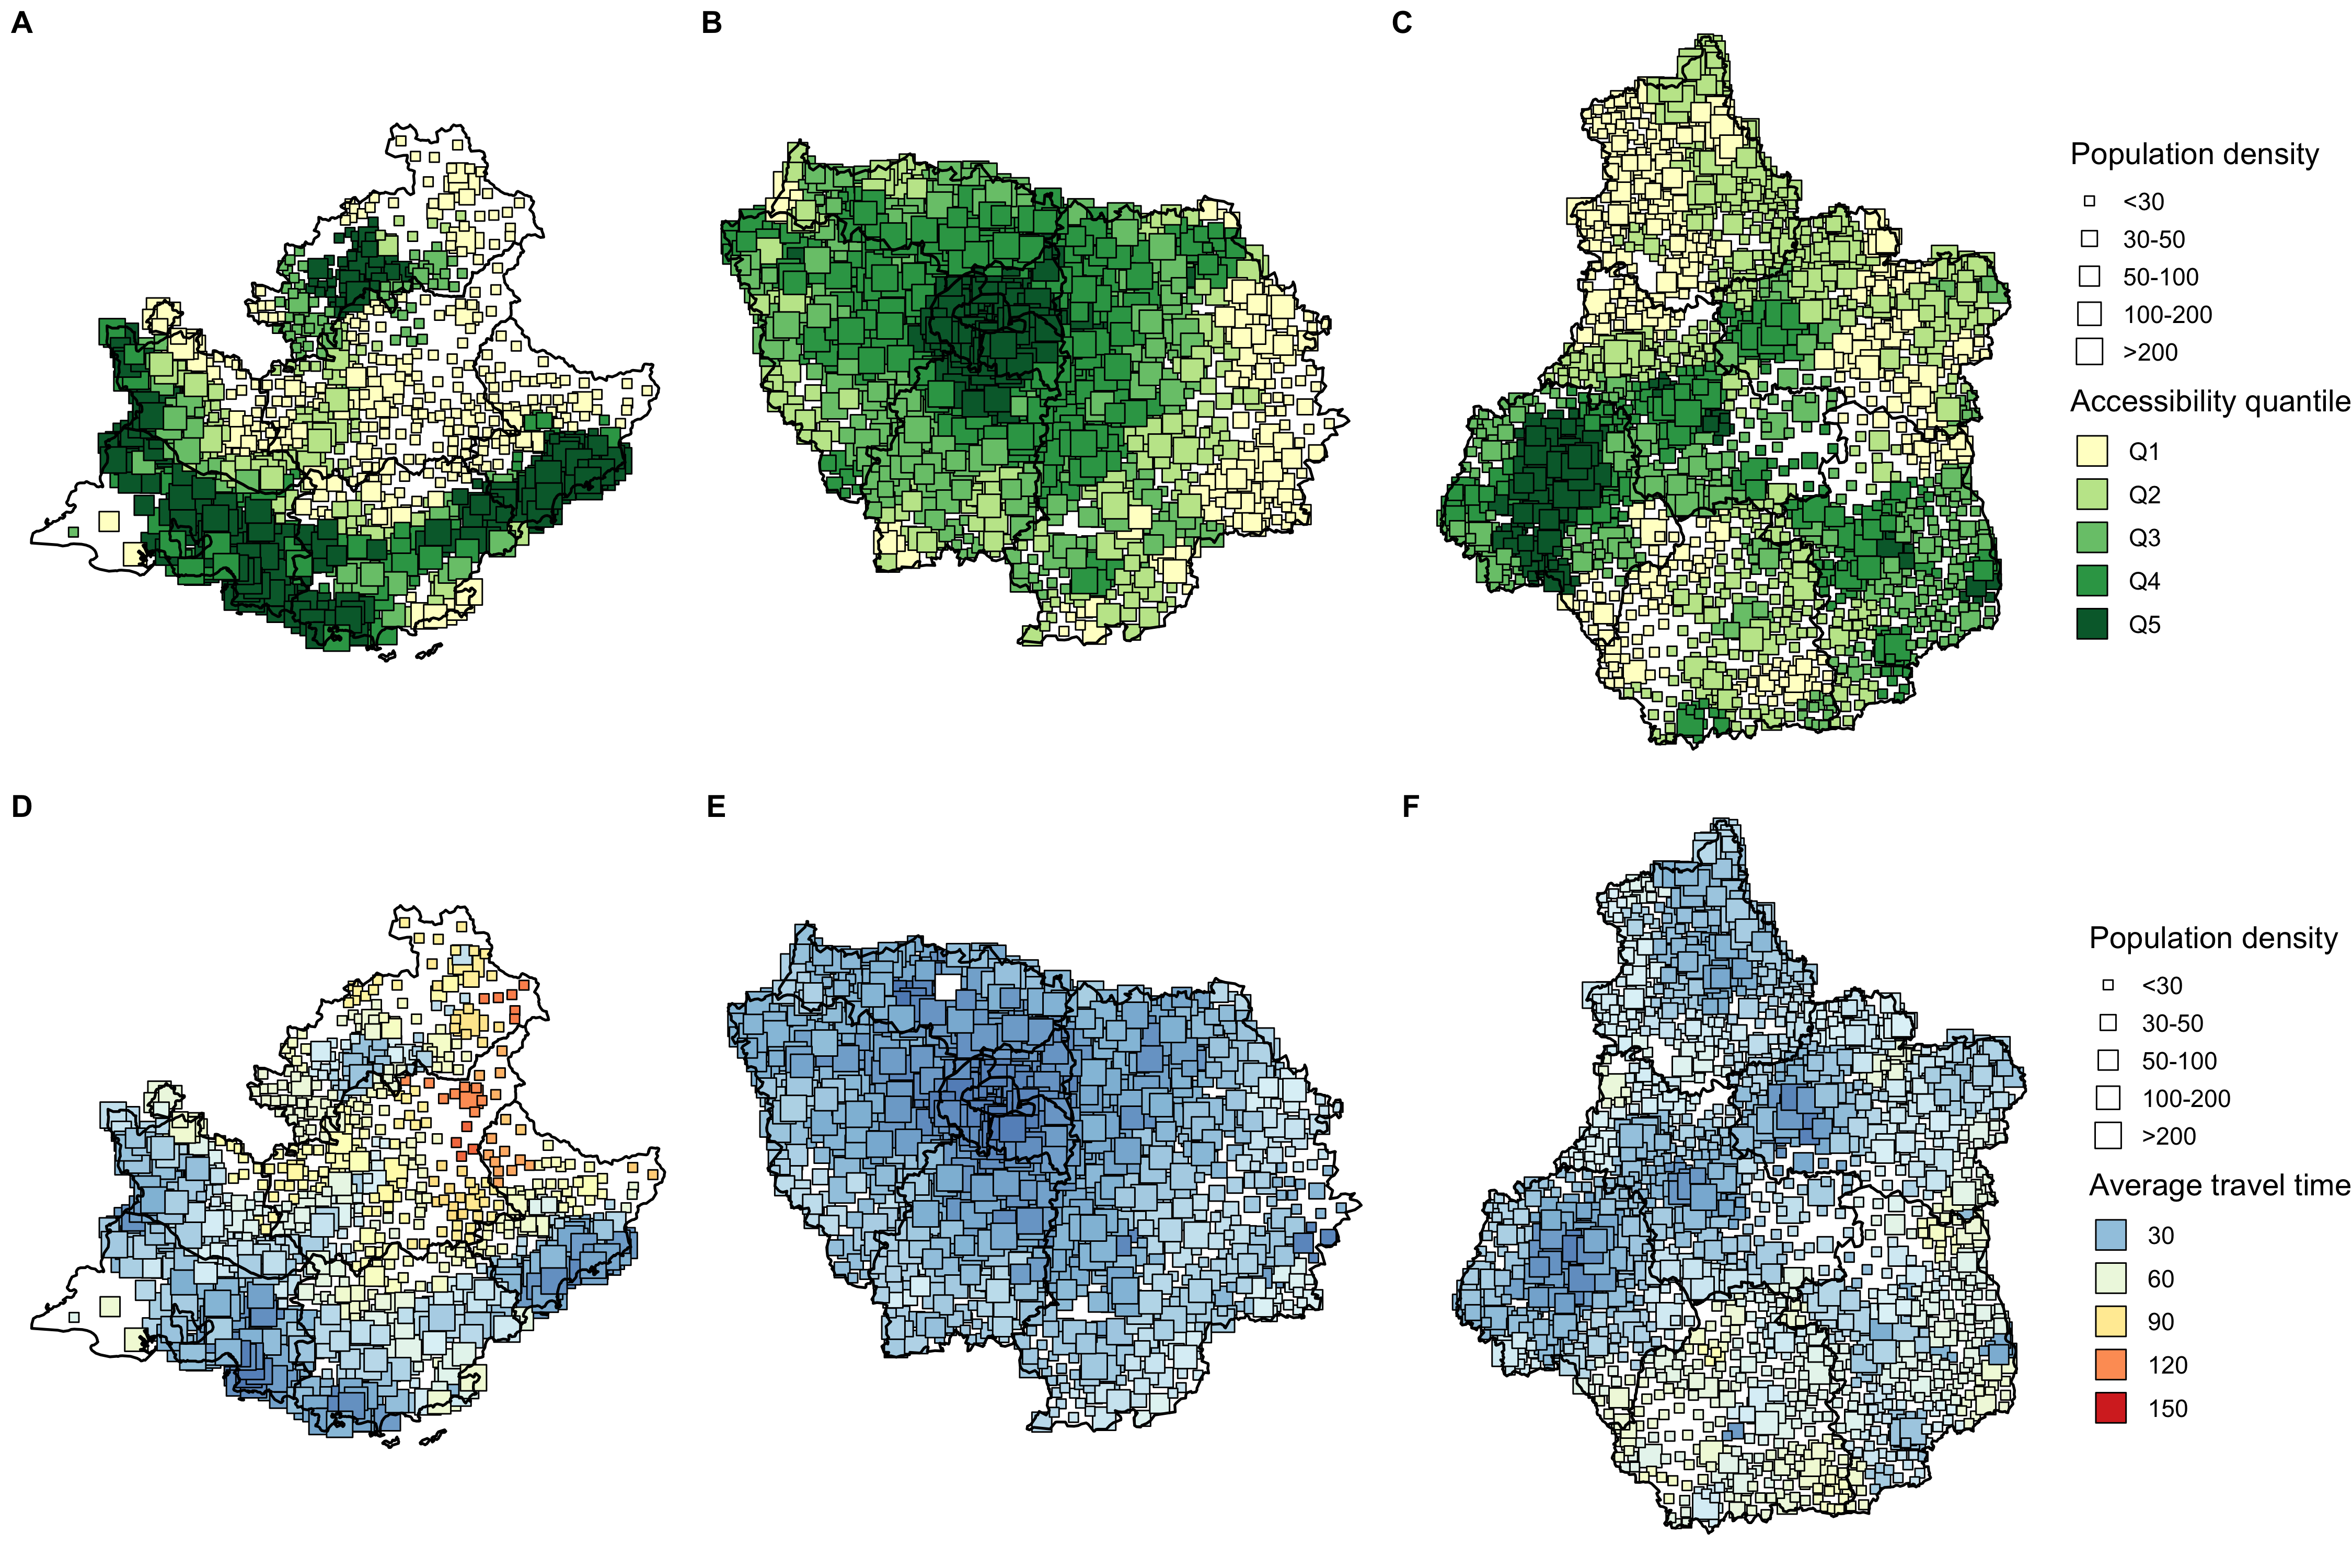
\includegraphics[width=\textwidth]{images/camion/fig3_accessibility_vs_density_scatter_map.png}
    \centering
    \caption{
        \textbf{Comparison of population density with accessibility scores and patient average travel time for cancer pathways.} Showing results in three regions: Provence-Alpes-Cote-d’Azur (A, D), Ile-de-France (B, E) and Bourgogne-Franche-Comté (C, F). Municipalities are drawn as squares, sized by population density and colored by either accessibility quantile (A, B, C) or patient average travel time (D, E, F).
    }
    \label{fig:accessibility-vs-density}
\end{figure}

Finally, we compared our accessibility score with the department exit ratio, by municipality. Department exit ratio is defined as the proportion of cancer patients who visited a care center outside from their department of residence and was computed using the \ac{pmsi} database. In Provence-Alpes-Cote-d'Azur, the exit ratio is higher in departments with low accessibility scores and few oncology specialized care centers, as in Alpes-de-Haute-Provence and Hautes-Alpes. While the Var department has some oncology centers, exit ratio remains high since larger care centers are in Marseille and Nice.

\subsection*{Provence-Alpes-Cote-d'Azur}

We now focus on the region Provence-Alpes-Cote-d'Azur. This region is the far southeastern on the mainland. The region's population was 5,048 million in 2018. Its prefecture and largest city is Marseille. The region contains six departments. Bouches-du-Rhone, Var and Alpes-Maritimes are located on the coastline and gather the largest cities like Marseille, Nice, or Toulon. Alpes-de-Haute-Provence, Vaucluse, and Hautes-Alpes are inland departments, with a majority of rural and mountainous areas. Results are shown on \cref{fig:accessibility-paca}. By comparing maps (A) and (B), we confirm that the accessibility is maximum in denser areas of the region. Average patients travel time are displayed on map (C) and we drew the major roads (primary, motorway and truck) in red. The road system is well developed on the coast, rallying the larger cities of the region. However, driving from the rural areas in the Alps to the major cities is hard, resulting in higher travel times. The accessibility is unevenly spread within the departments, especially in Alpes-Maritimes where the distribution is multi-modal (D). There, cities like Nice and Cannes have large hospitals thus good accessibility, while the northern areas of the department are mostly mountains. Accessibility is higher in municipalities with dense populations, for all the departments (E). Finally, the average travel time decreases when the accessibility score increases. This makes sense since the accessibility score was computed based on the driving distance between population locations and care centers. However, it confirms that patients living in poor accessibility zones effectively travel further to seek oncology care. In Bouches-du-Rhone, nearly all the municipalities have an average travel time lower than 30 minutes, while in Alpes-de-Haute-Provence, average travel times are rarely lower than 60 minutes (F).

\begin{figure}[H]
    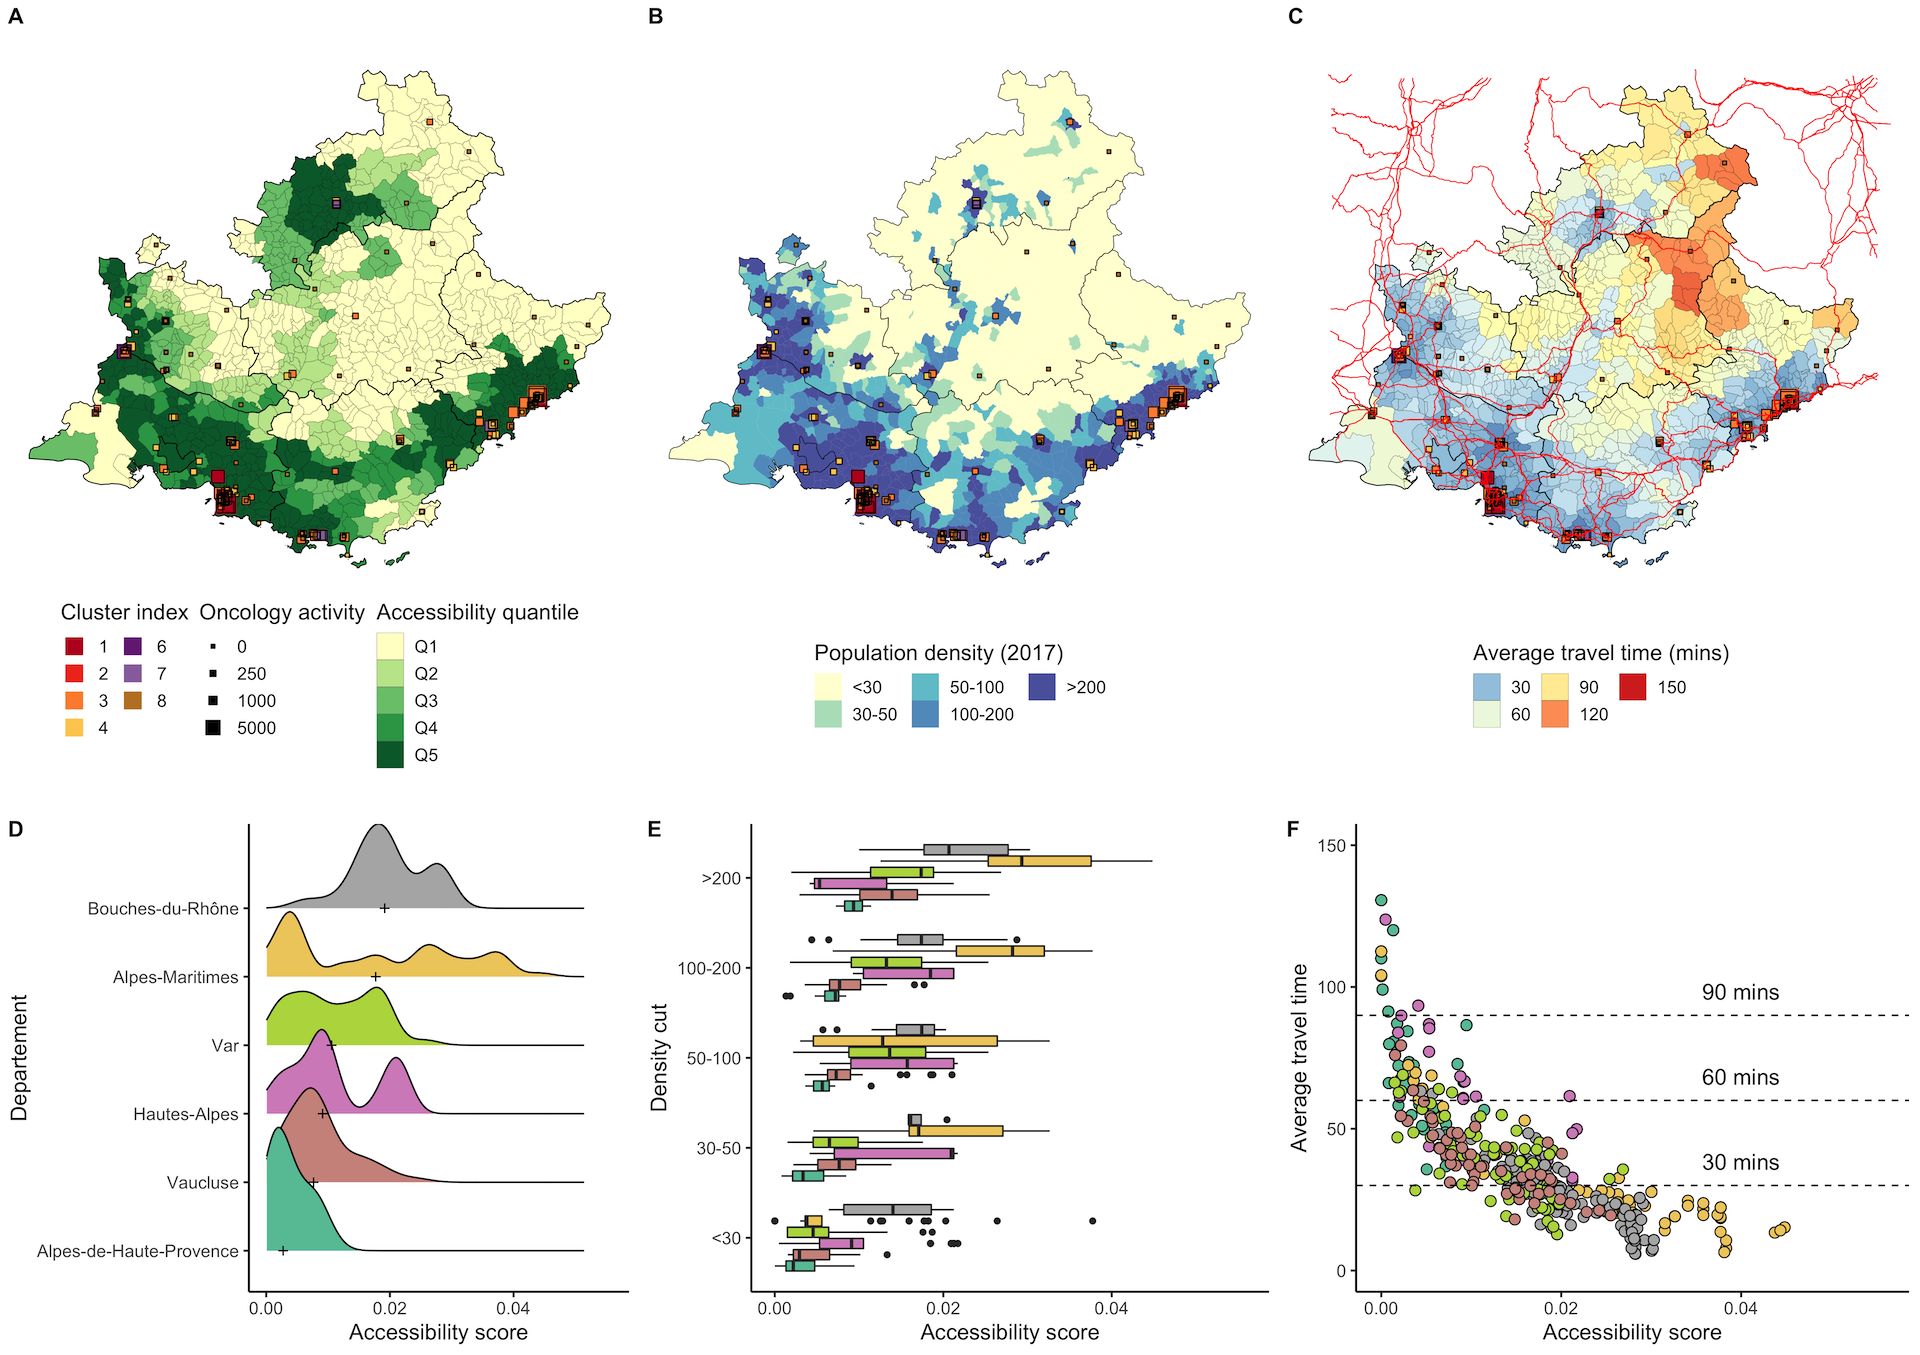
\includegraphics[width=\textwidth]{images/camion/fig4_accessibility_Provence-Alpes-Cote-d'Azur.png}
    \centering
    \caption{
        \textbf{Accessibility distribution in Provence-Alpes-Cote-d'Azur region.} Map (A) shows the region accessibility distribution per municipality. Map (B) displays the population density discretized in 5 bins. The map on plot (C) displays the average travel time for cancer pathways. Large roads (primary, motorway and trucks) are drawn in red. Plot (D) shows the accessibility distribution per department of the region. Plot (E) shows the accessibility distribution by municipality population density and department. Plot (F) compares the accessibility score from municipalities with the average travel time for cancer pathways.
    }
    \label{fig:accessibility-paca}
\end{figure}

\subsection*{Pays de la Loire}

\begin{figure}[H]
    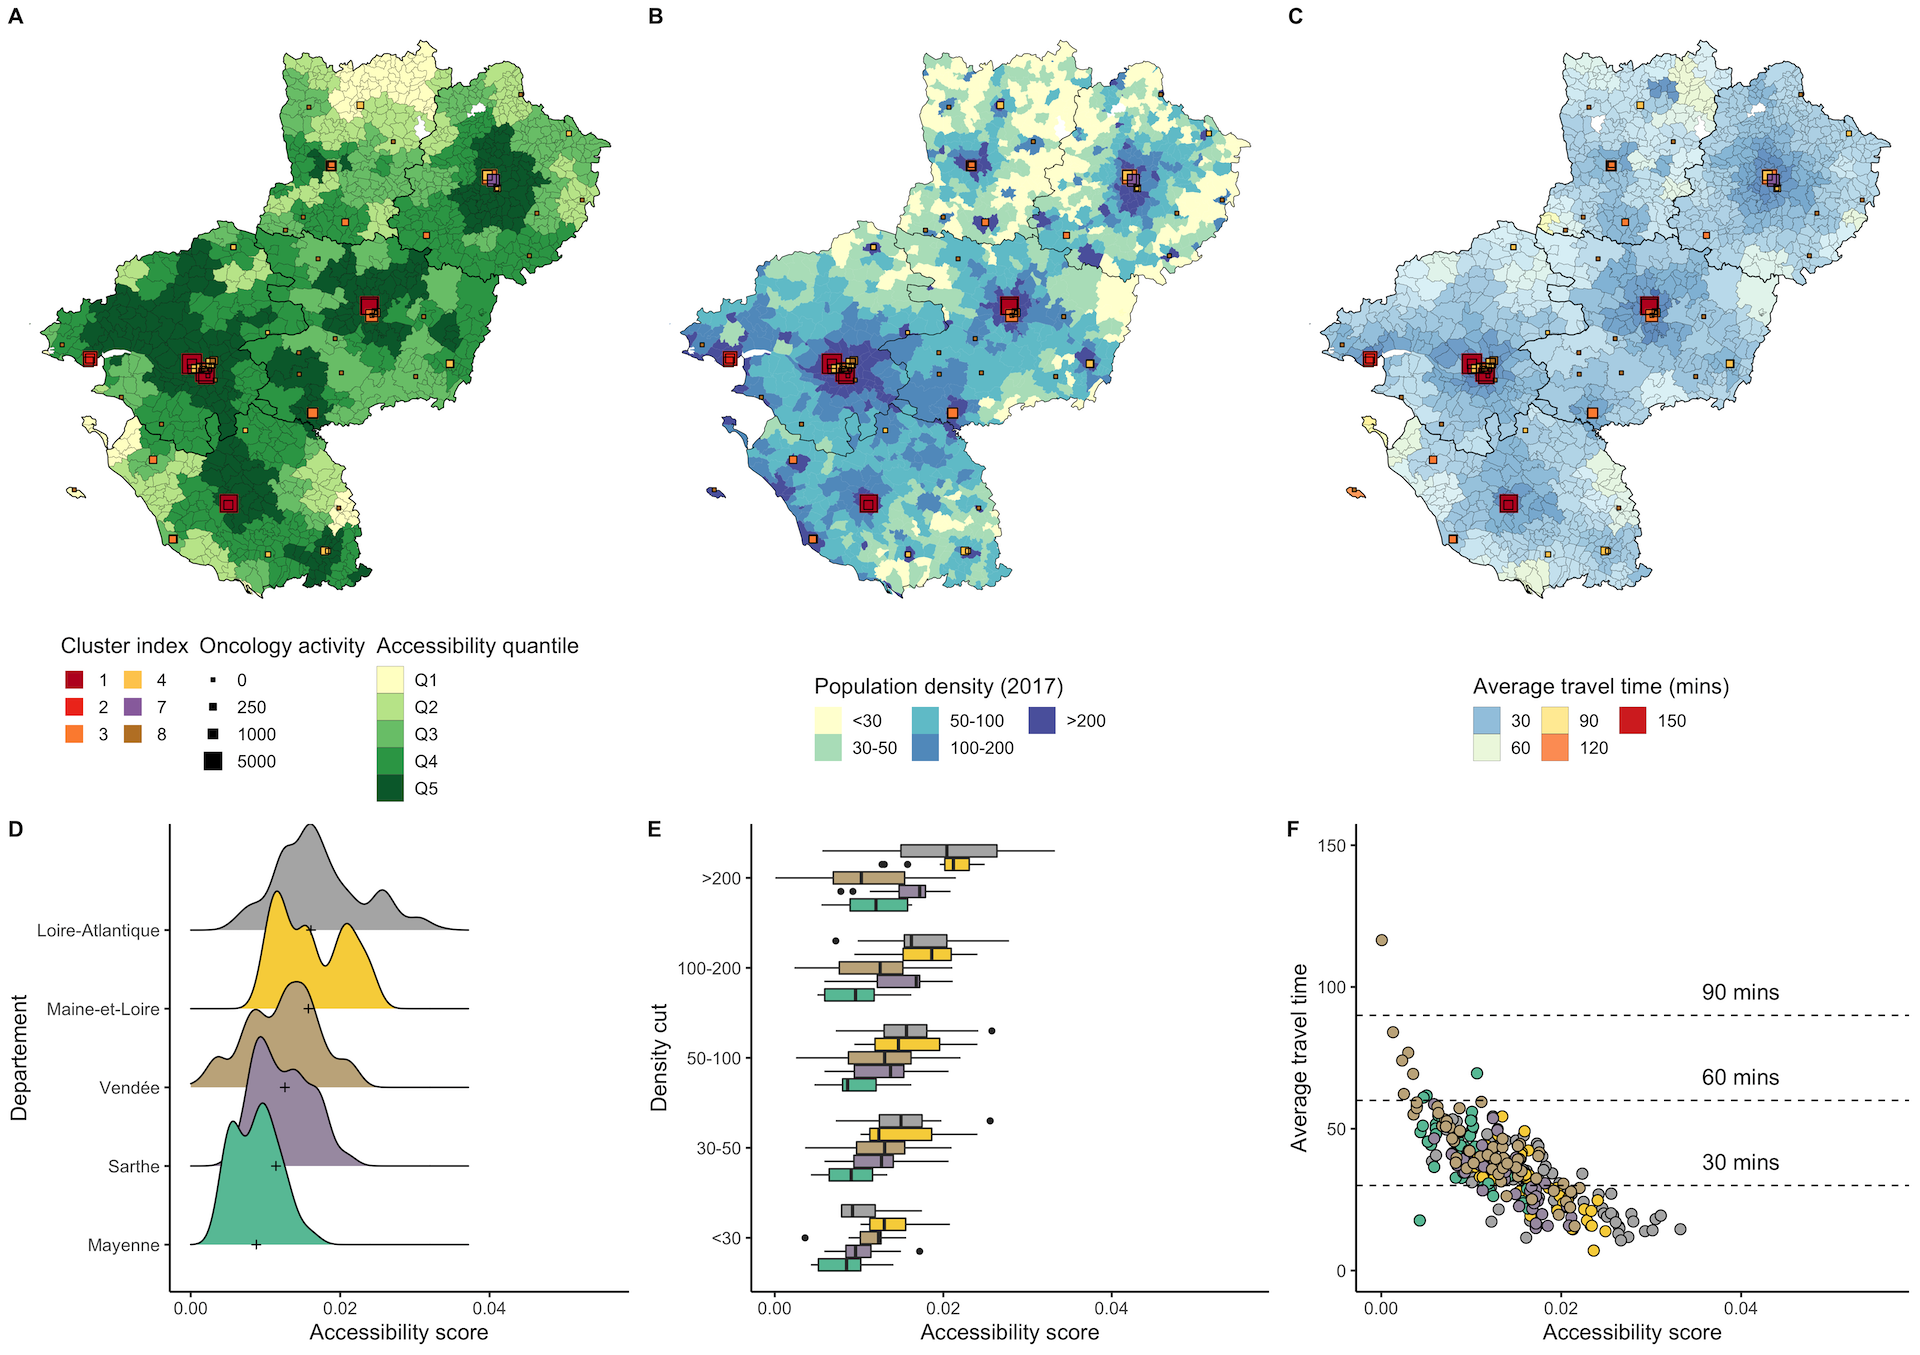
\includegraphics[width=\textwidth]{images/camion/region_accessibility/accessibility_Pays-de-la-Loire.png}
    \centering
    \caption{
        \textbf{Accessibility distribution in Pays-de-la-Loire.}
    }
\end{figure}

\subsection*{Occitanie}

\begin{figure}[H]
    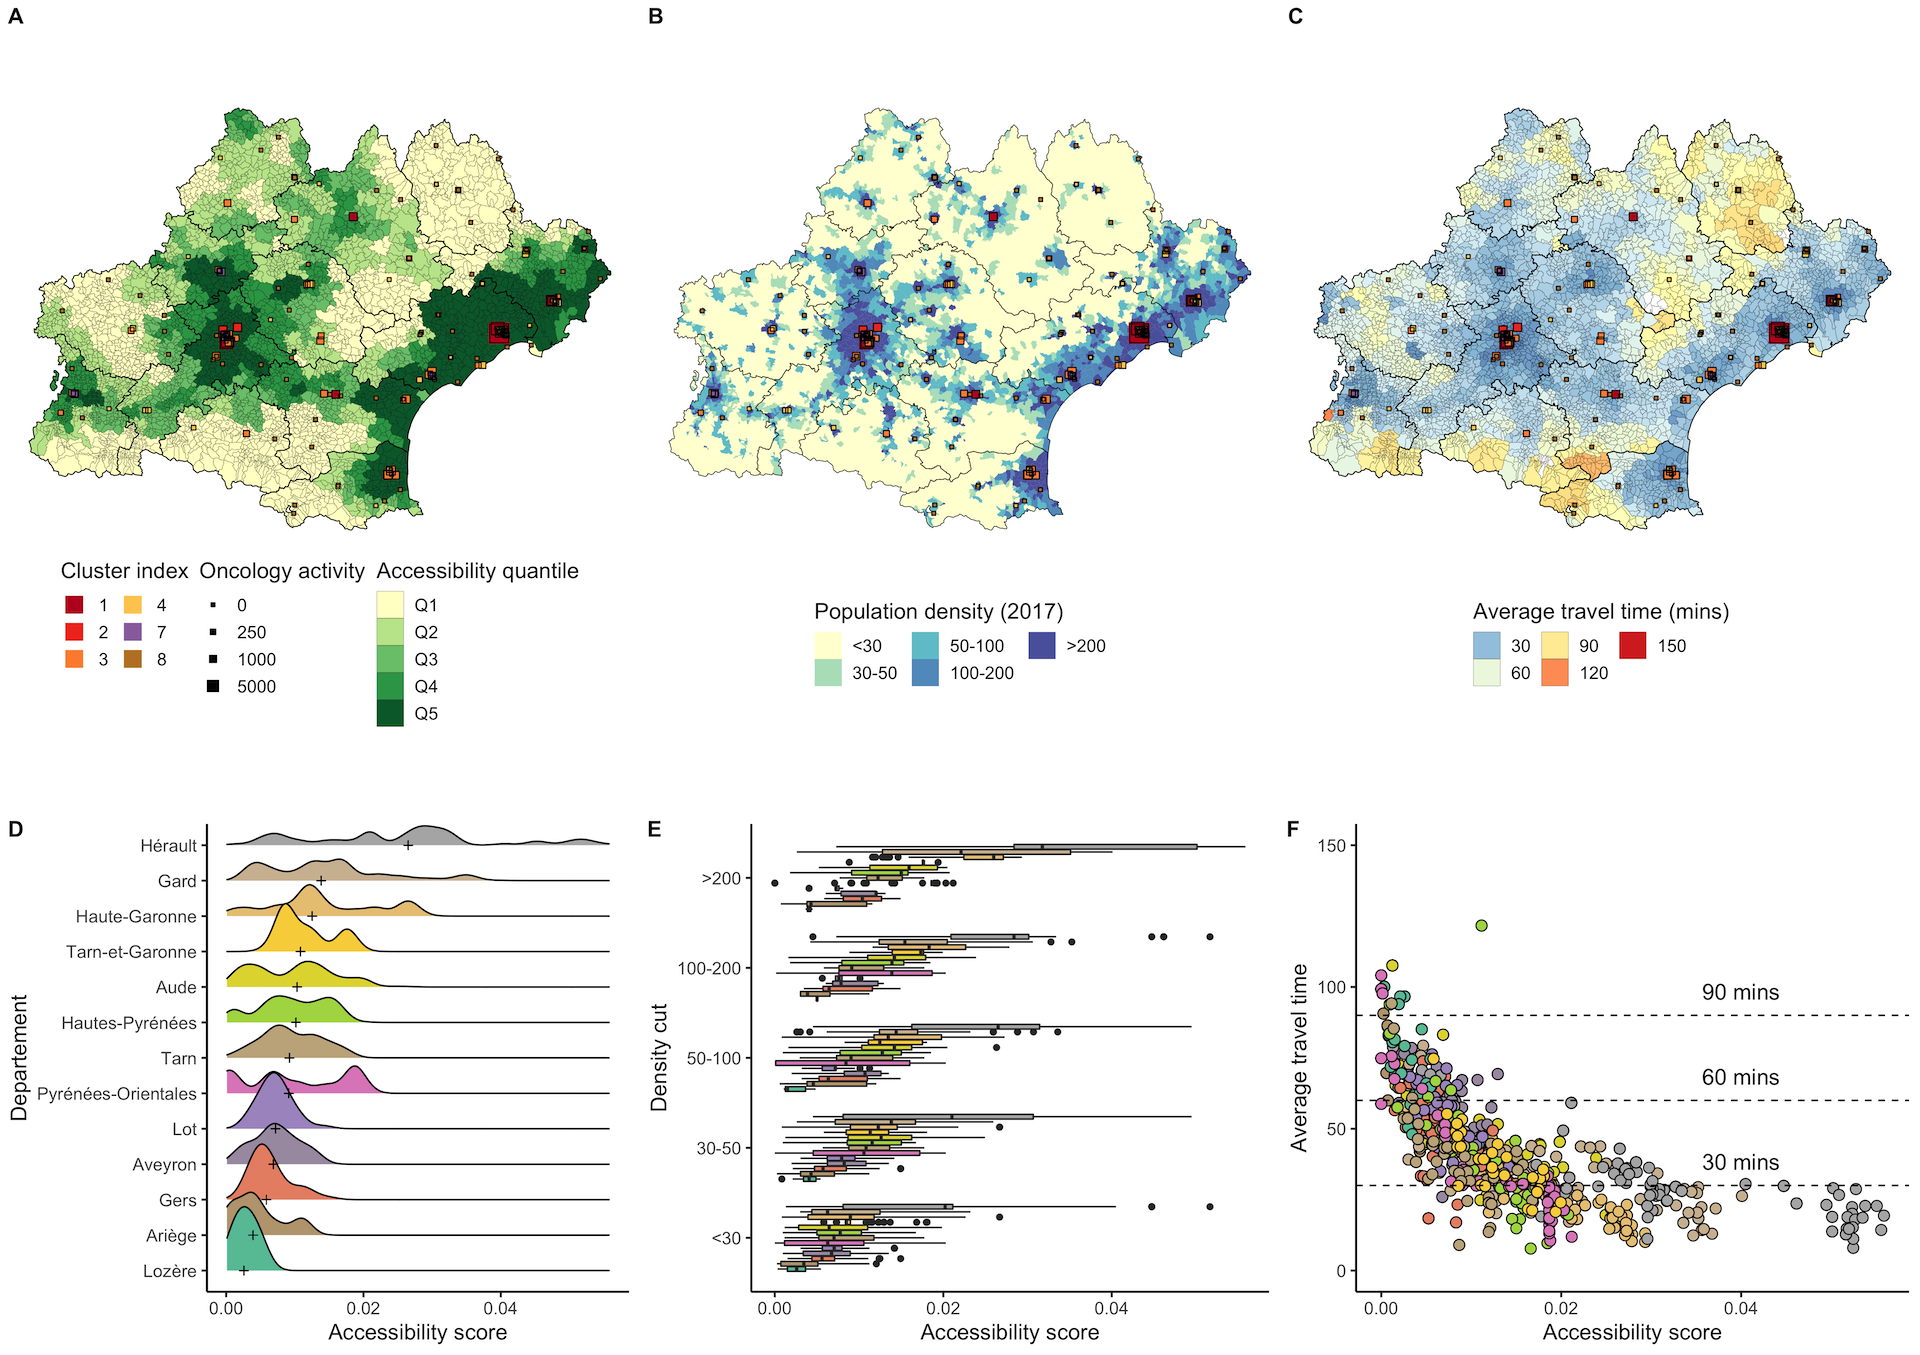
\includegraphics[width=\textwidth]{images/camion/region_accessibility/accessibility_Occitanie.png}
    \centering
    \caption{
        \textbf{Accessibility distribution in Occitanie.}
    }
\end{figure}

\subsection*{Nouvelle-Aquitaine}

\begin{figure}[H]
    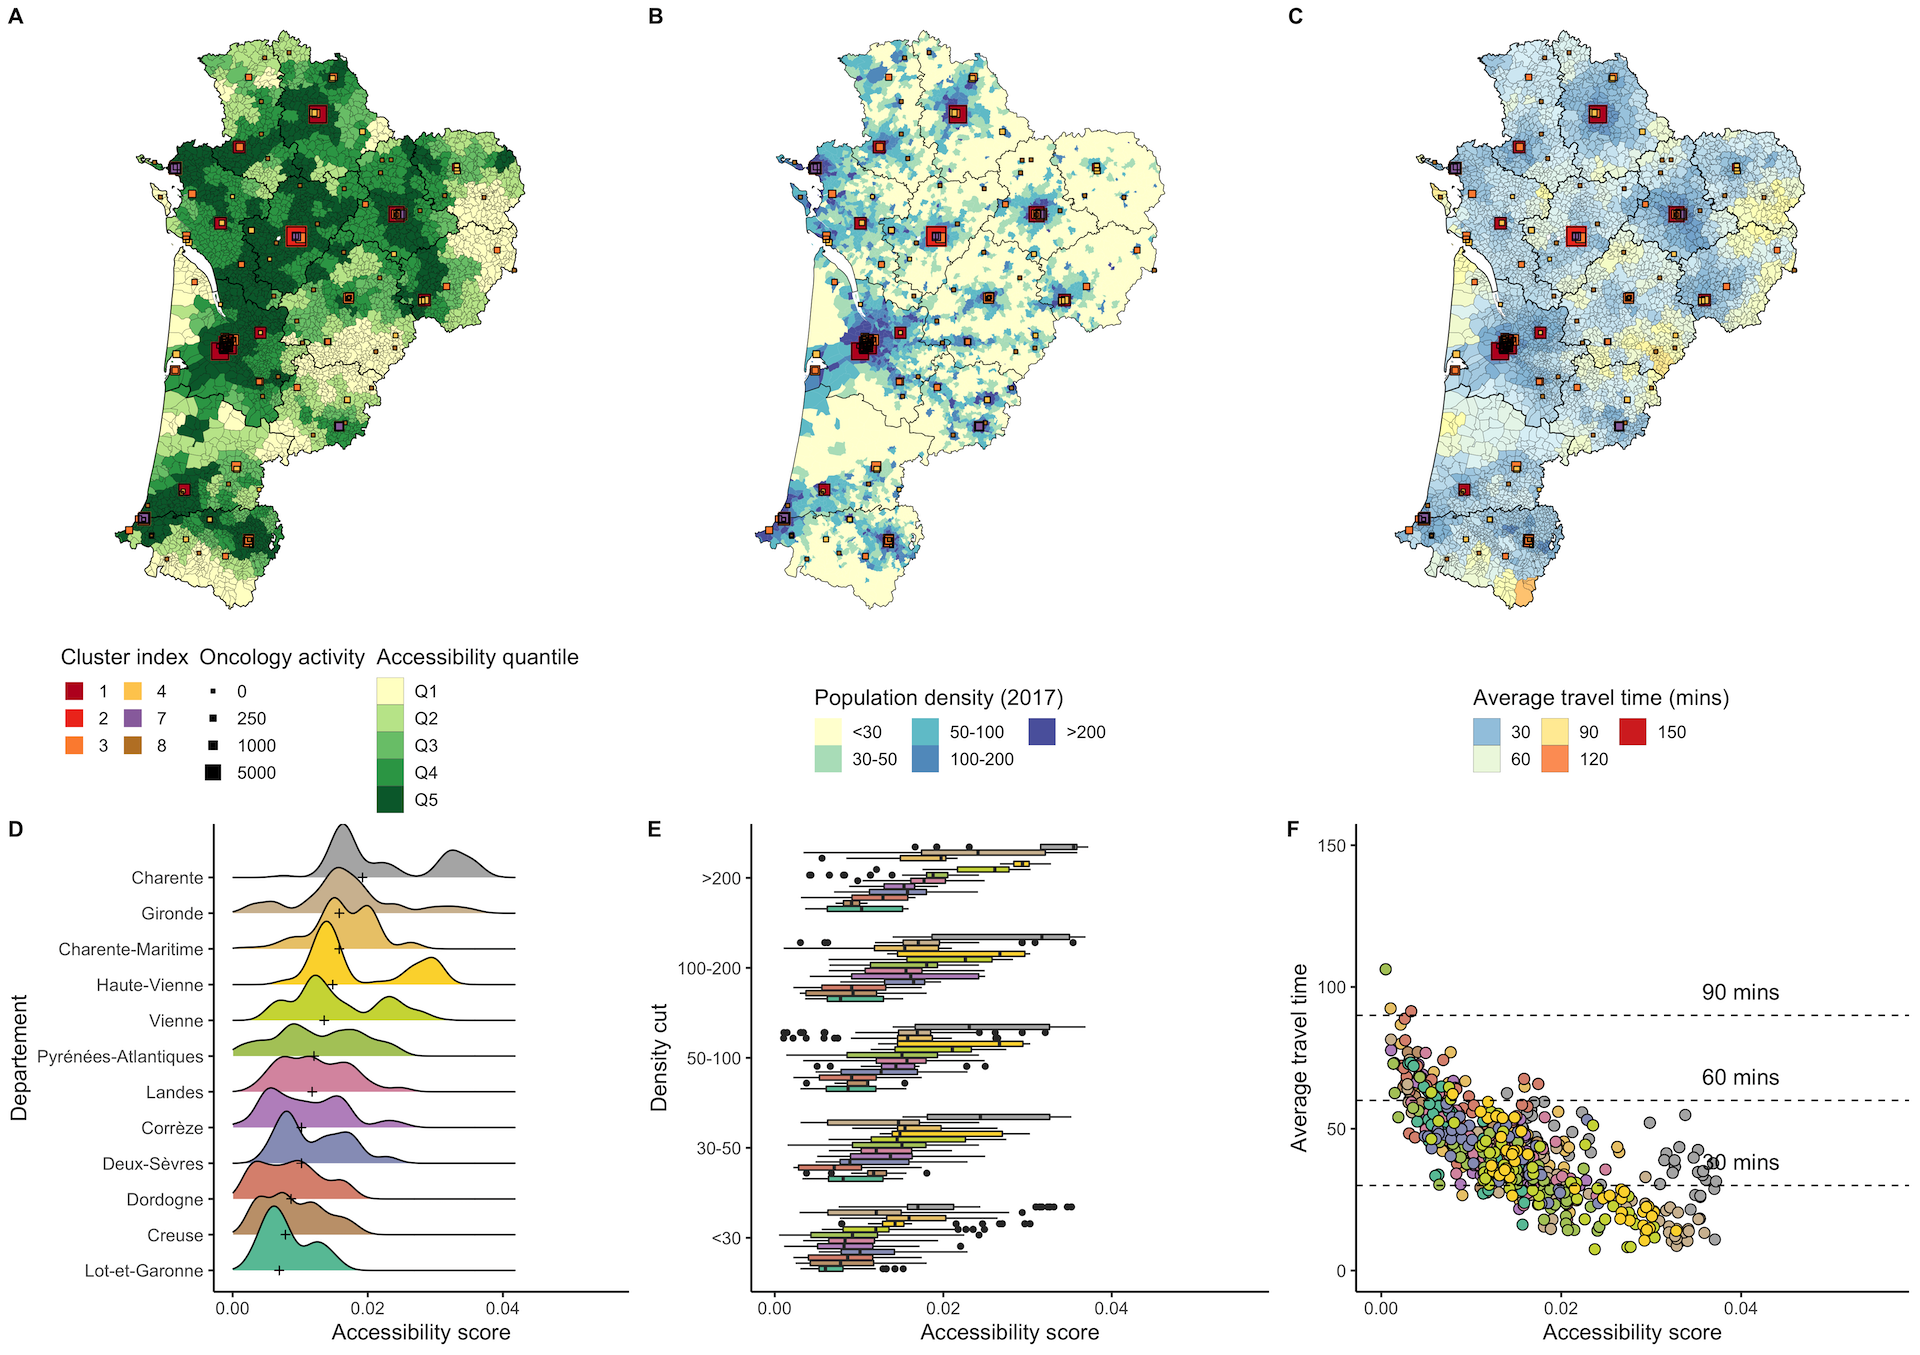
\includegraphics[width=\textwidth]{images/camion/region_accessibility/accessibility_Nouvelle-Aquitaine.png}
    \centering
    \caption{
        \textbf{Accessibility distribution in Nouvelle-Aquitaine.}
    }
\end{figure}

\subsection*{Normandie}

\begin{figure}[H]
    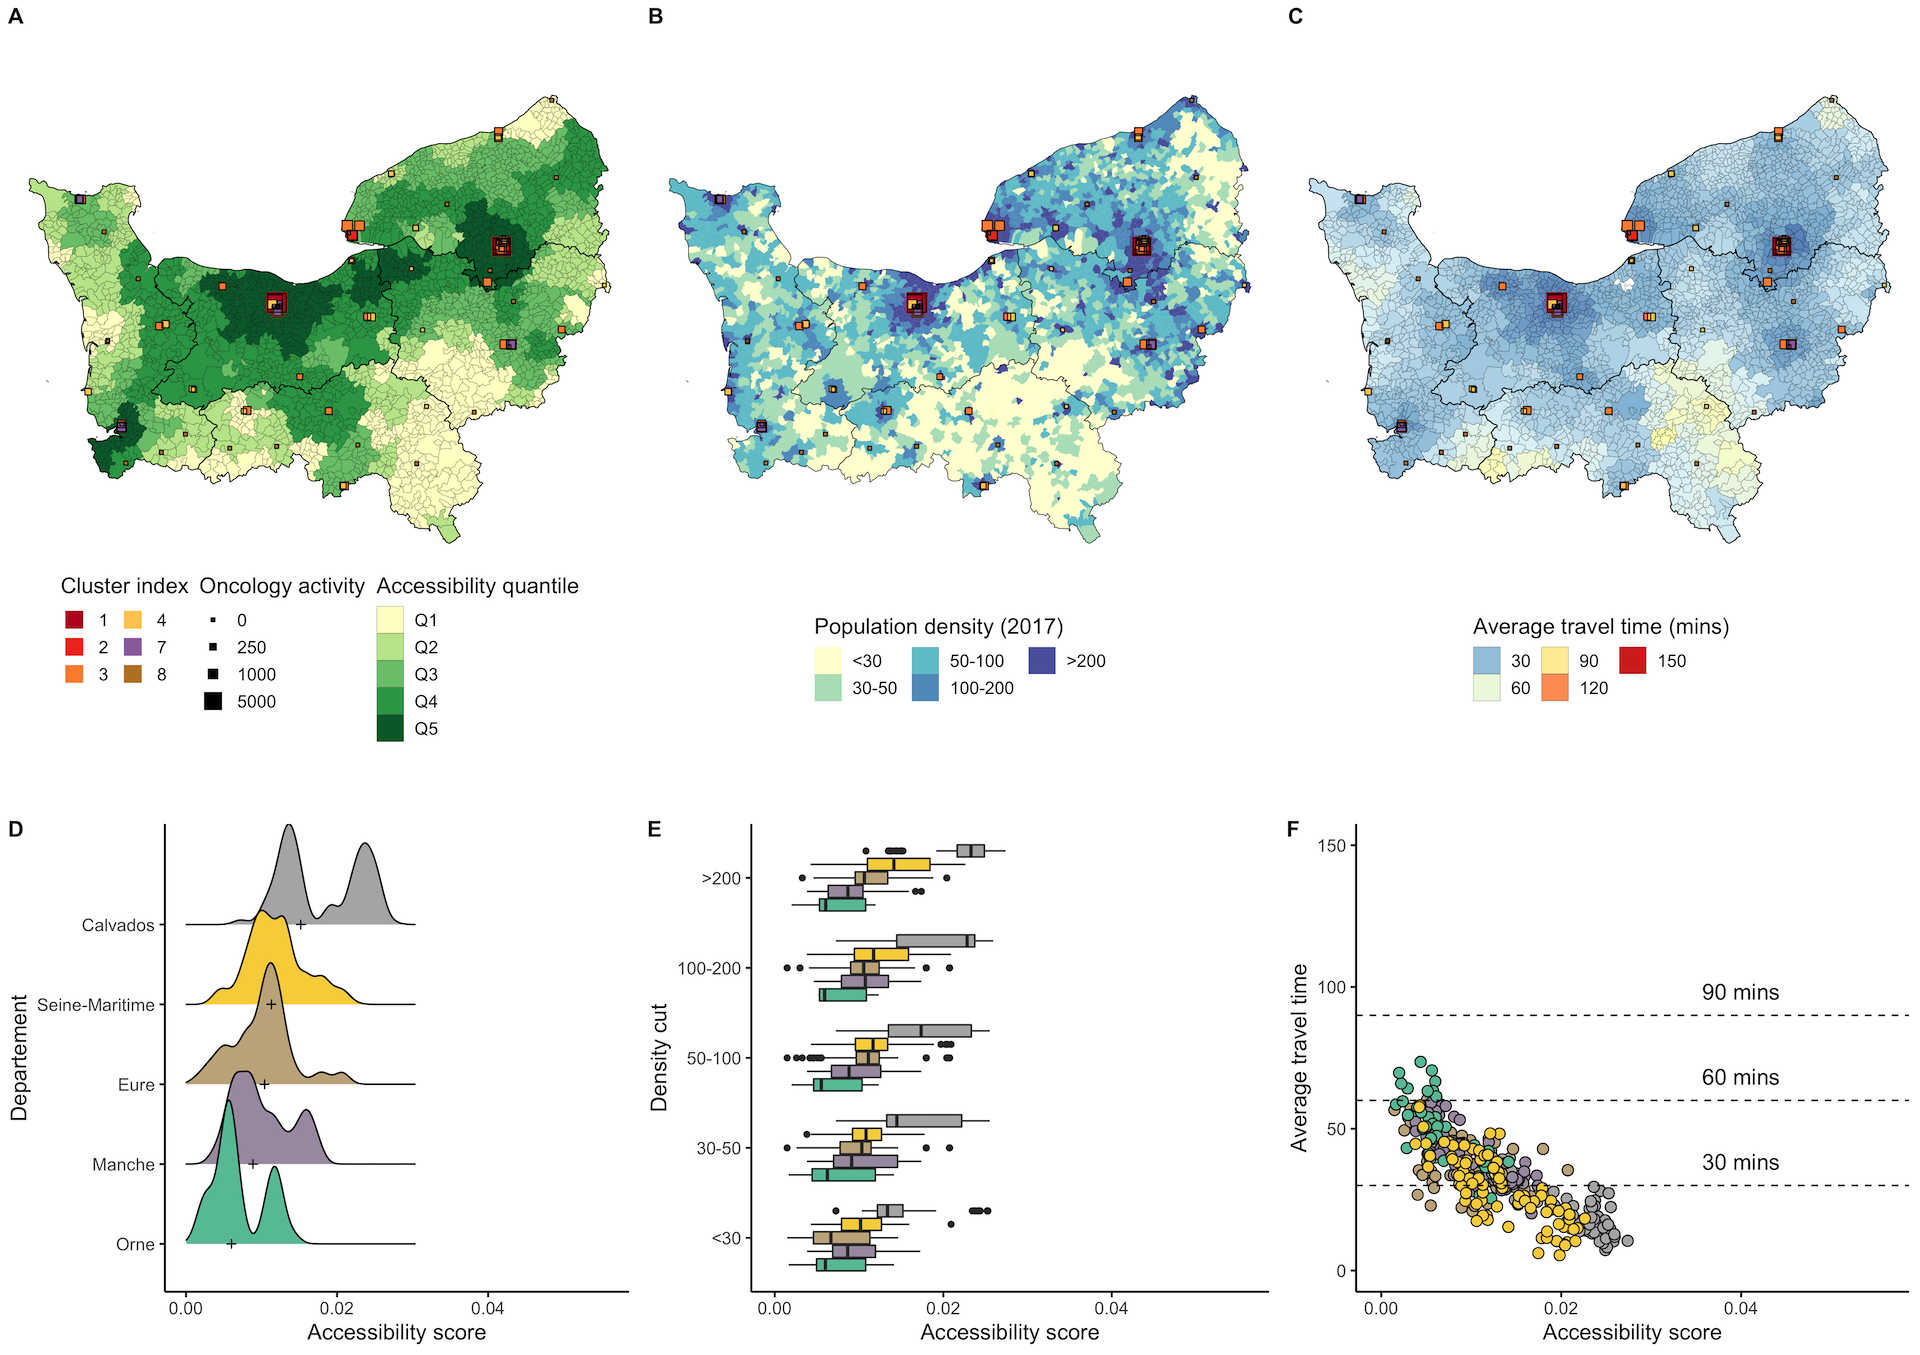
\includegraphics[width=\textwidth]{images/camion/region_accessibility/accessibility_Normandie.png}
    \centering
    \caption{
        \textbf{Accessibility distribution in Normandie.}
    }
\end{figure}

\subsection*{Île-de-France}

\begin{figure}[H]
    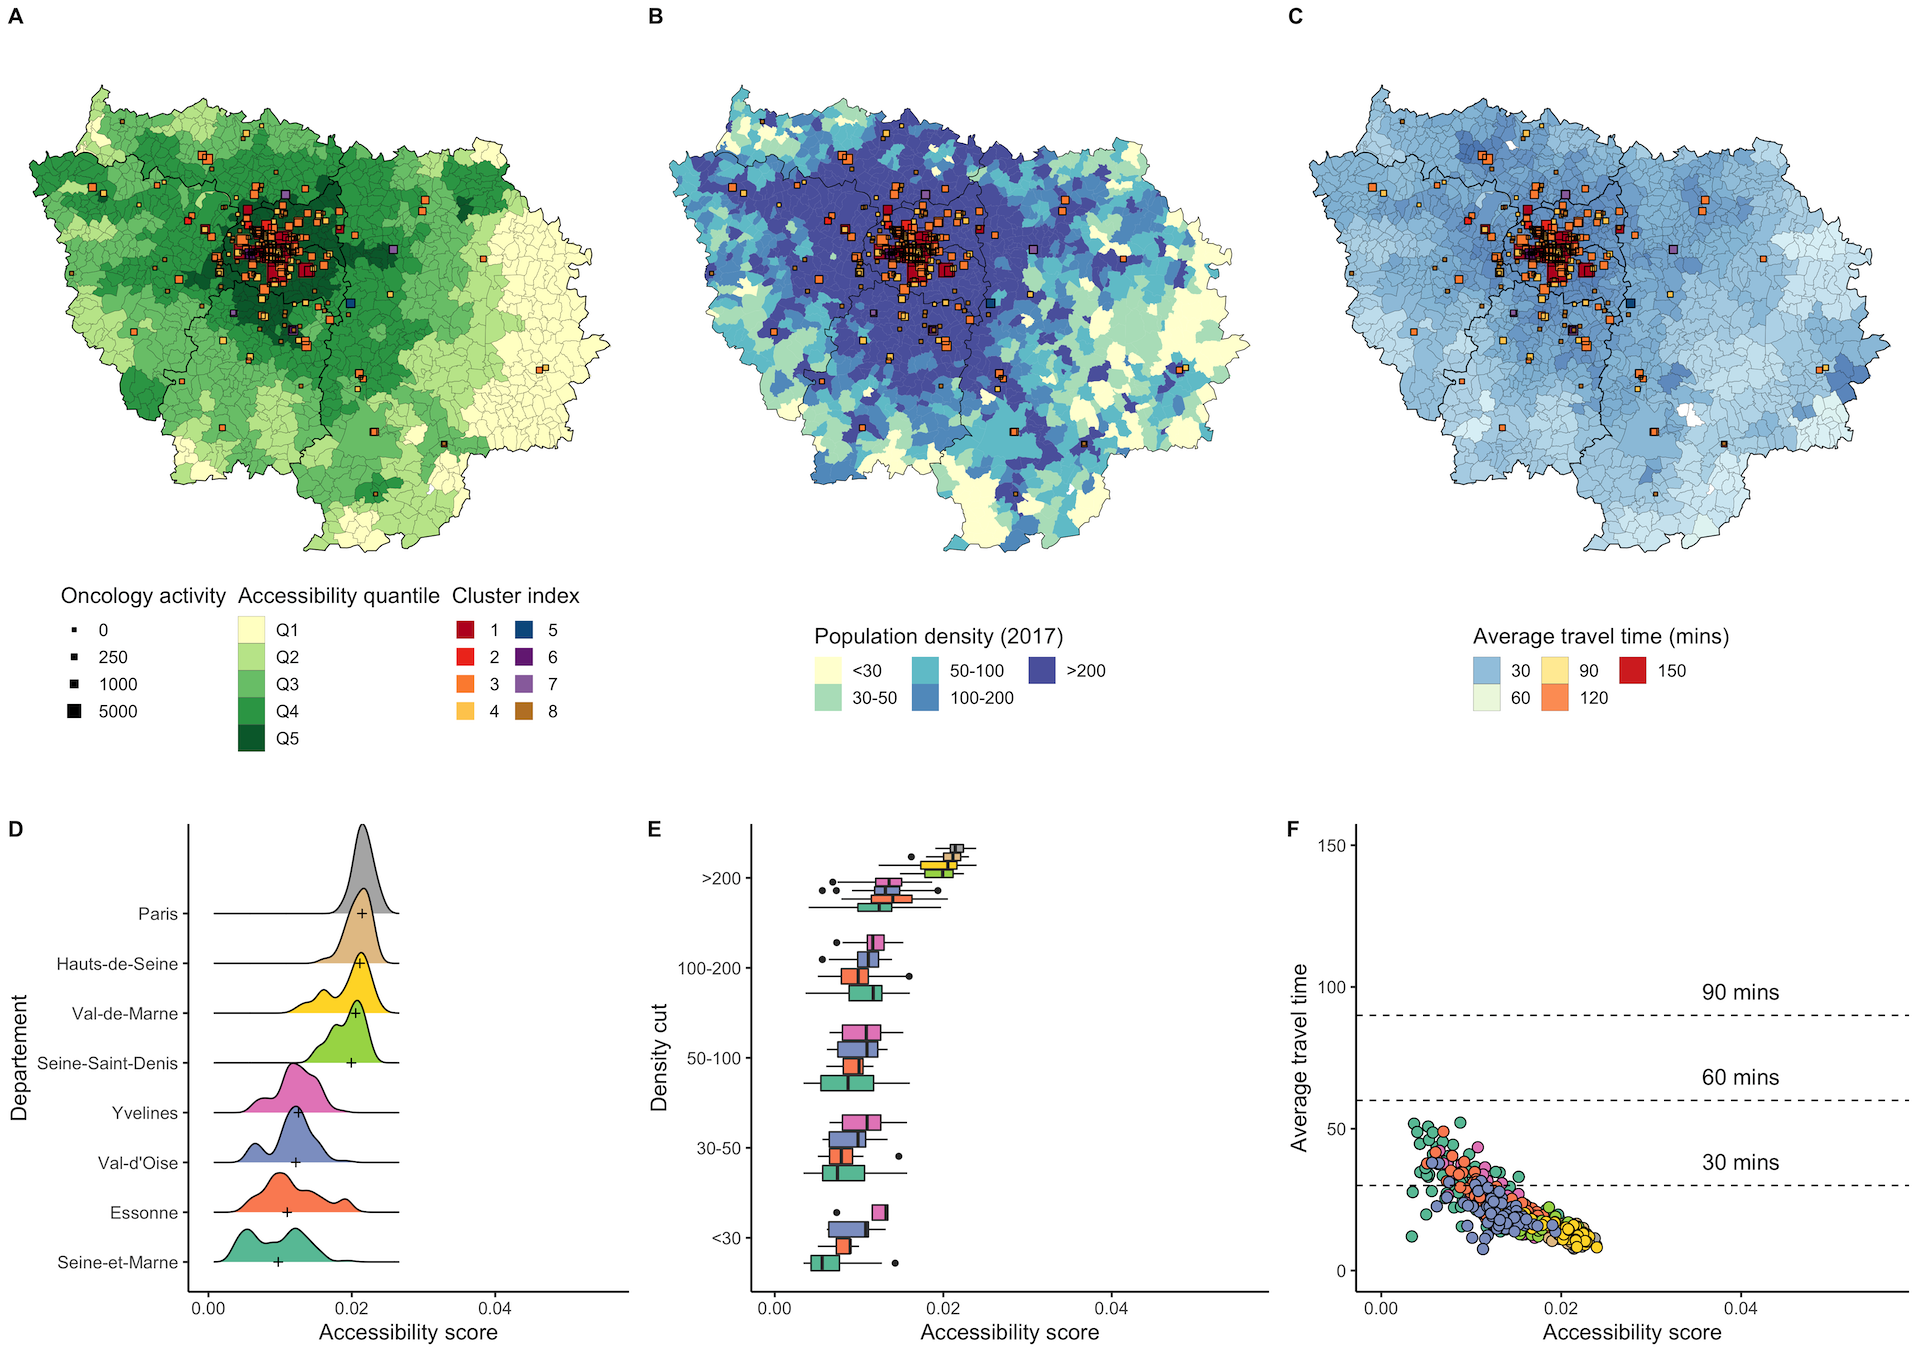
\includegraphics[width=\textwidth]{images/camion/region_accessibility/accessibility_Ile-de-France.png}
    \centering
    \caption{
        \textbf{Accessibility distribution in Ile-de-France.}
    }
\end{figure}

\subsection*{Hauts-de-France}

\begin{figure}[H]
    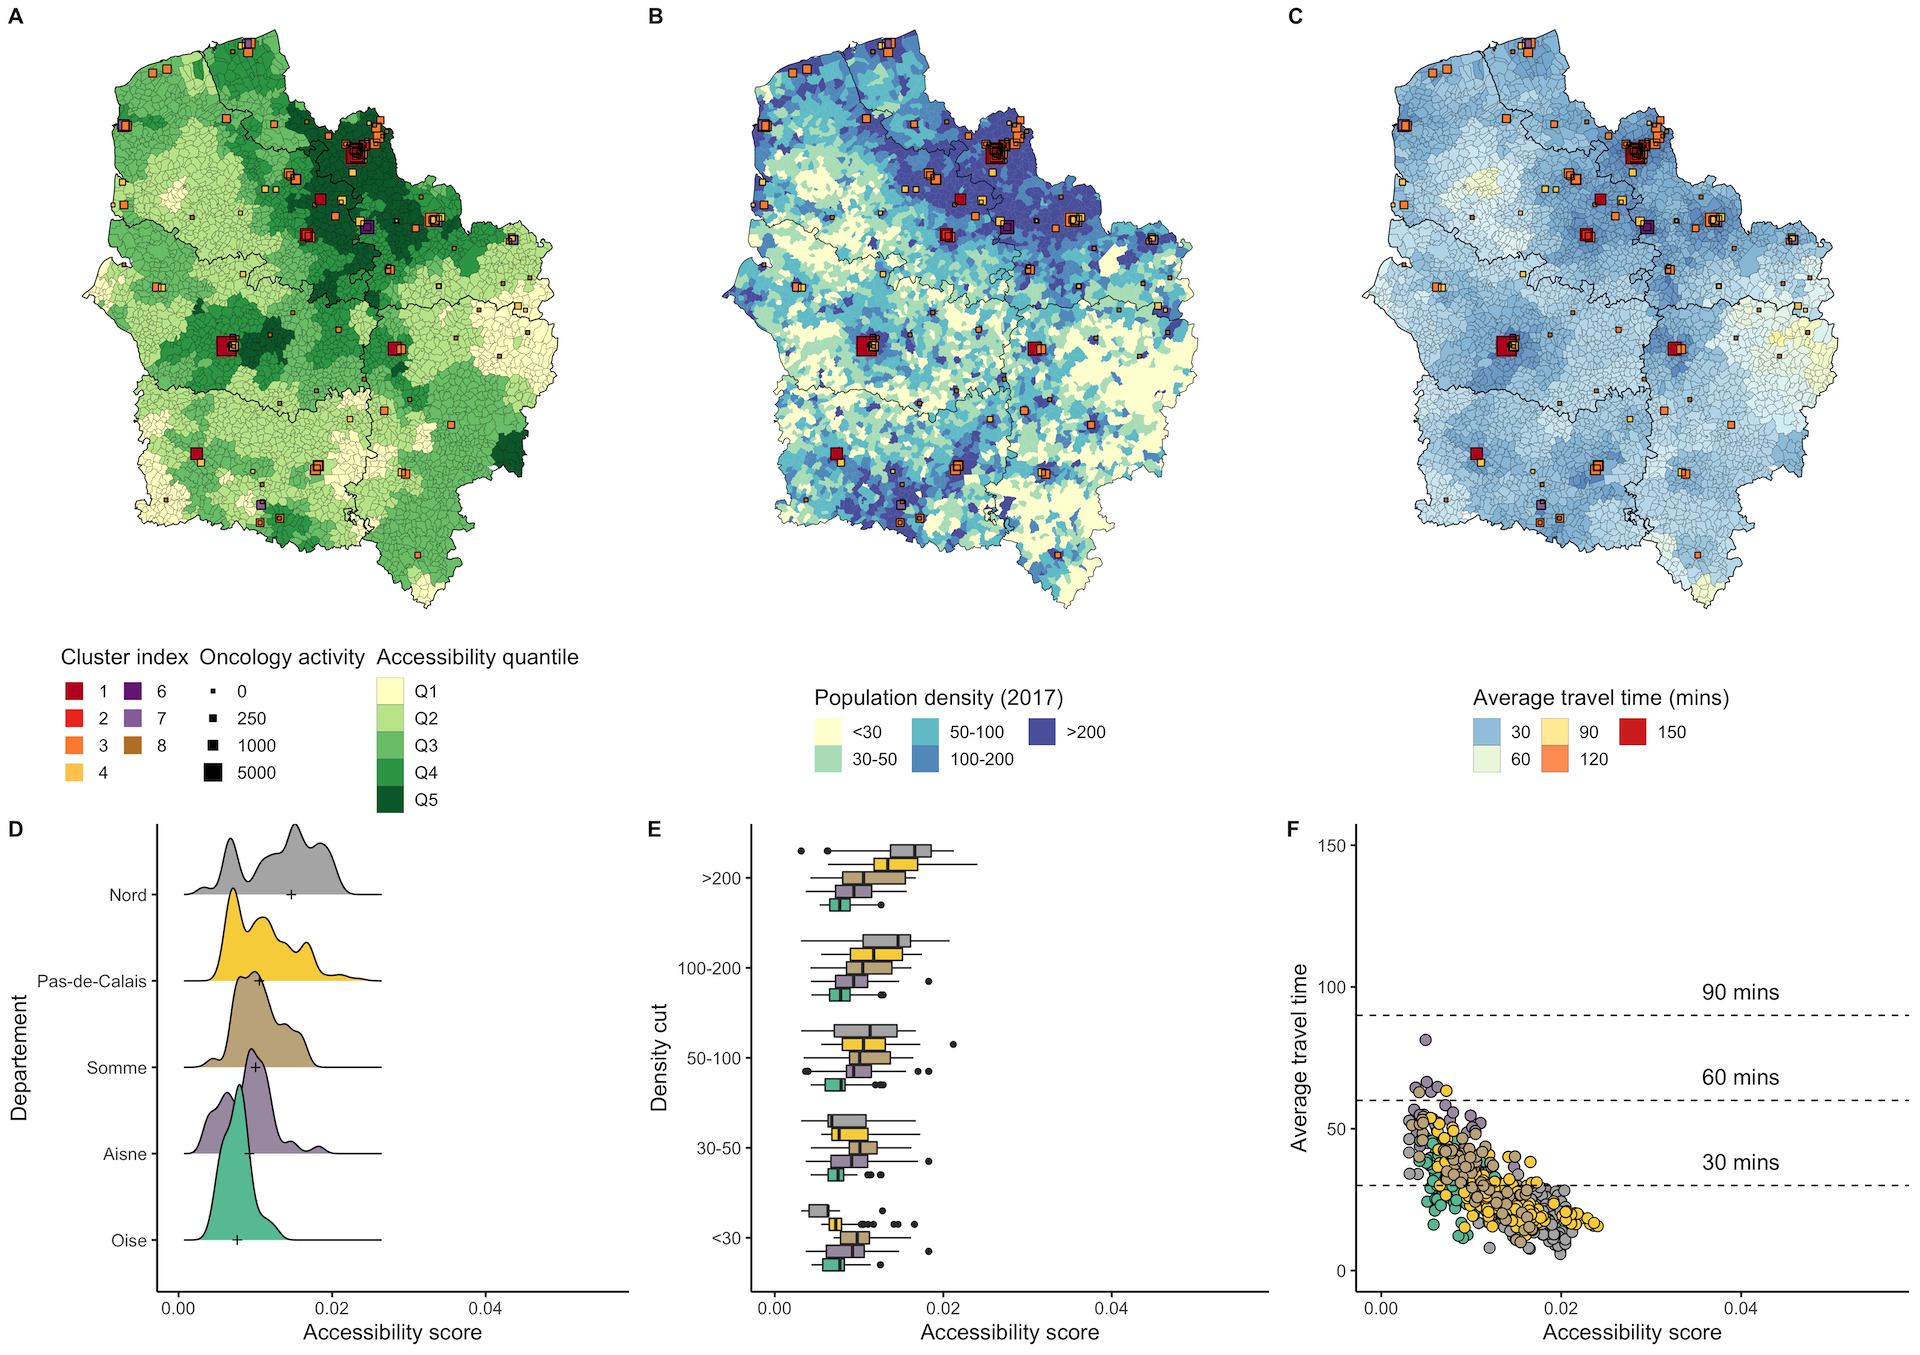
\includegraphics[width=\textwidth]{images/camion/region_accessibility/accessibility_Hauts-de-France.png}
    \centering
    \caption{
        \textbf{Accessibility distribution in Hauts-de-France.}
    }
\end{figure}

\subsection*{Grand Est}

\begin{figure}[H]
    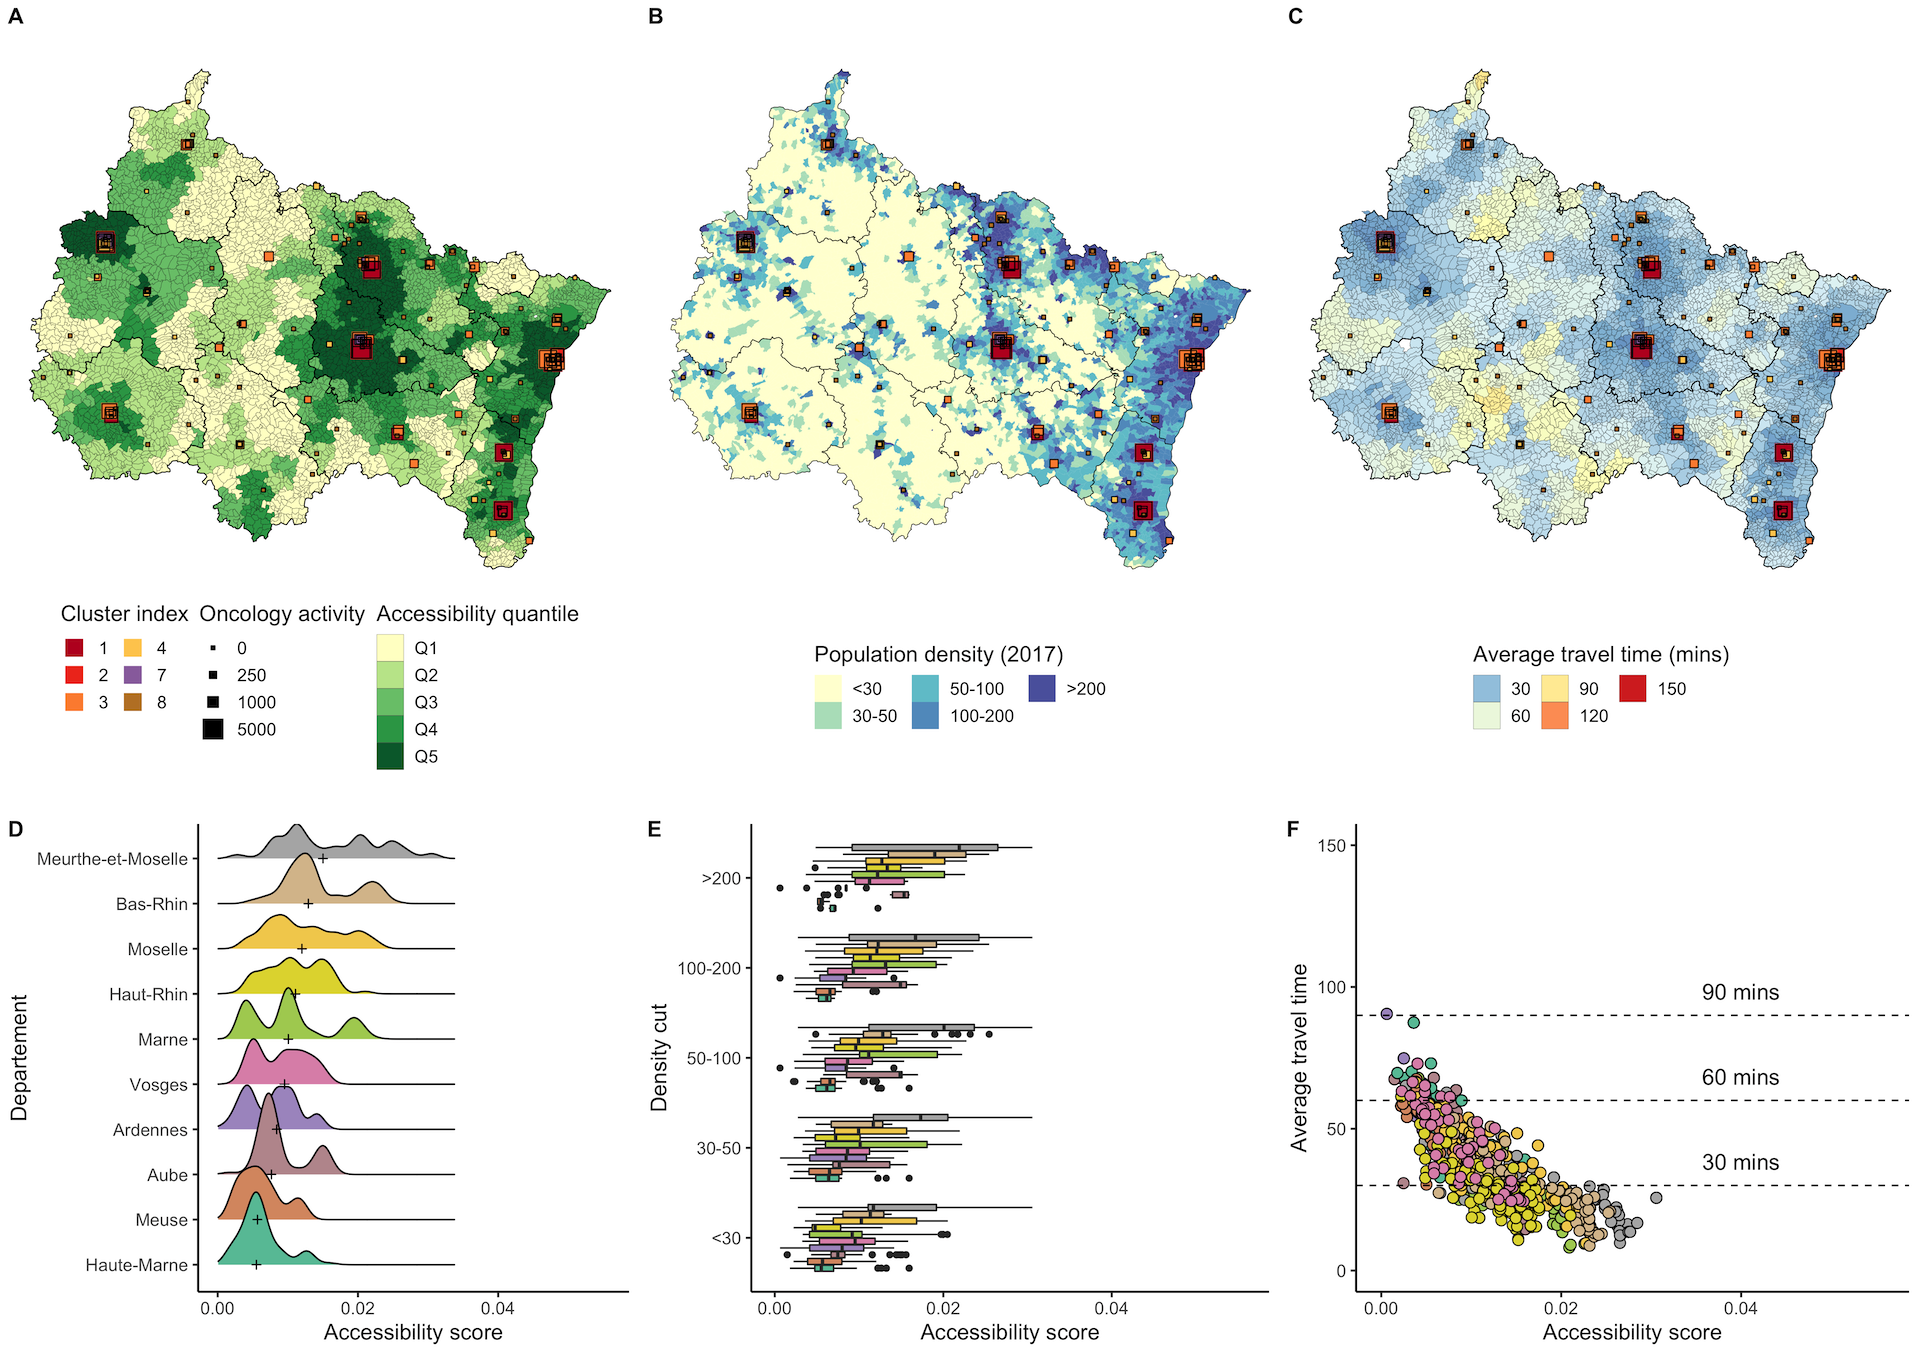
\includegraphics[width=\textwidth]{images/camion/region_accessibility/accessibility_Grand-Est.png}
    \centering
    \caption{
        \textbf{Accessibility distribution in Grand-Est.}
    }
\end{figure}

\subsection*{Centre-Val de Loire}

\begin{figure}[H]
    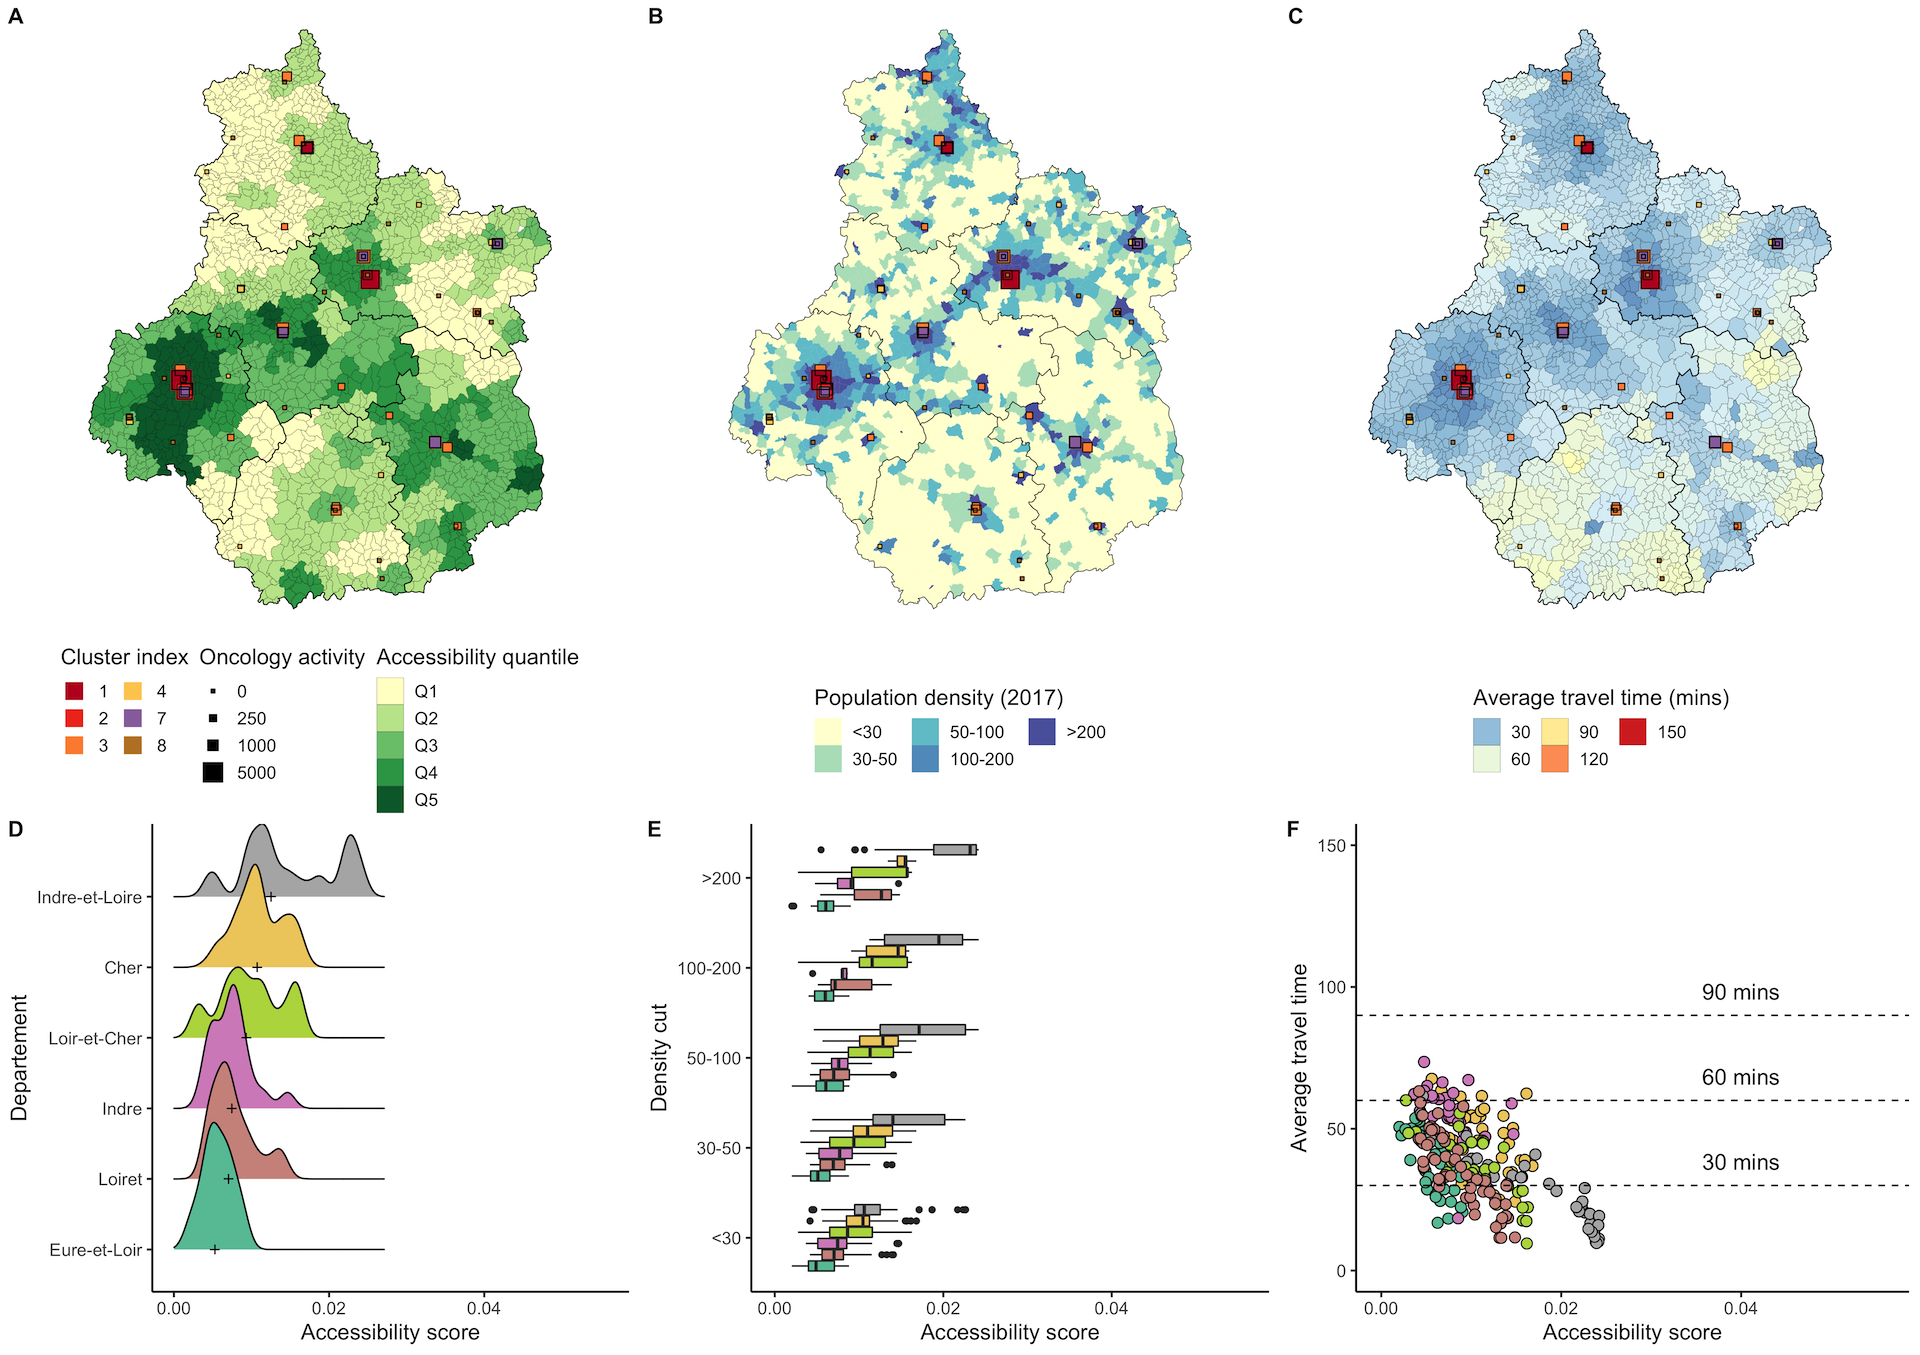
\includegraphics[width=\textwidth]{images/camion/region_accessibility/accessibility_Centre-Val-de-Loire.png}
    \centering
    \caption{
        \textbf{Accessibility distribution in Centre Val de Loire.}
    }
\end{figure}

\subsection*{Bretagne}

\begin{figure}[H]
    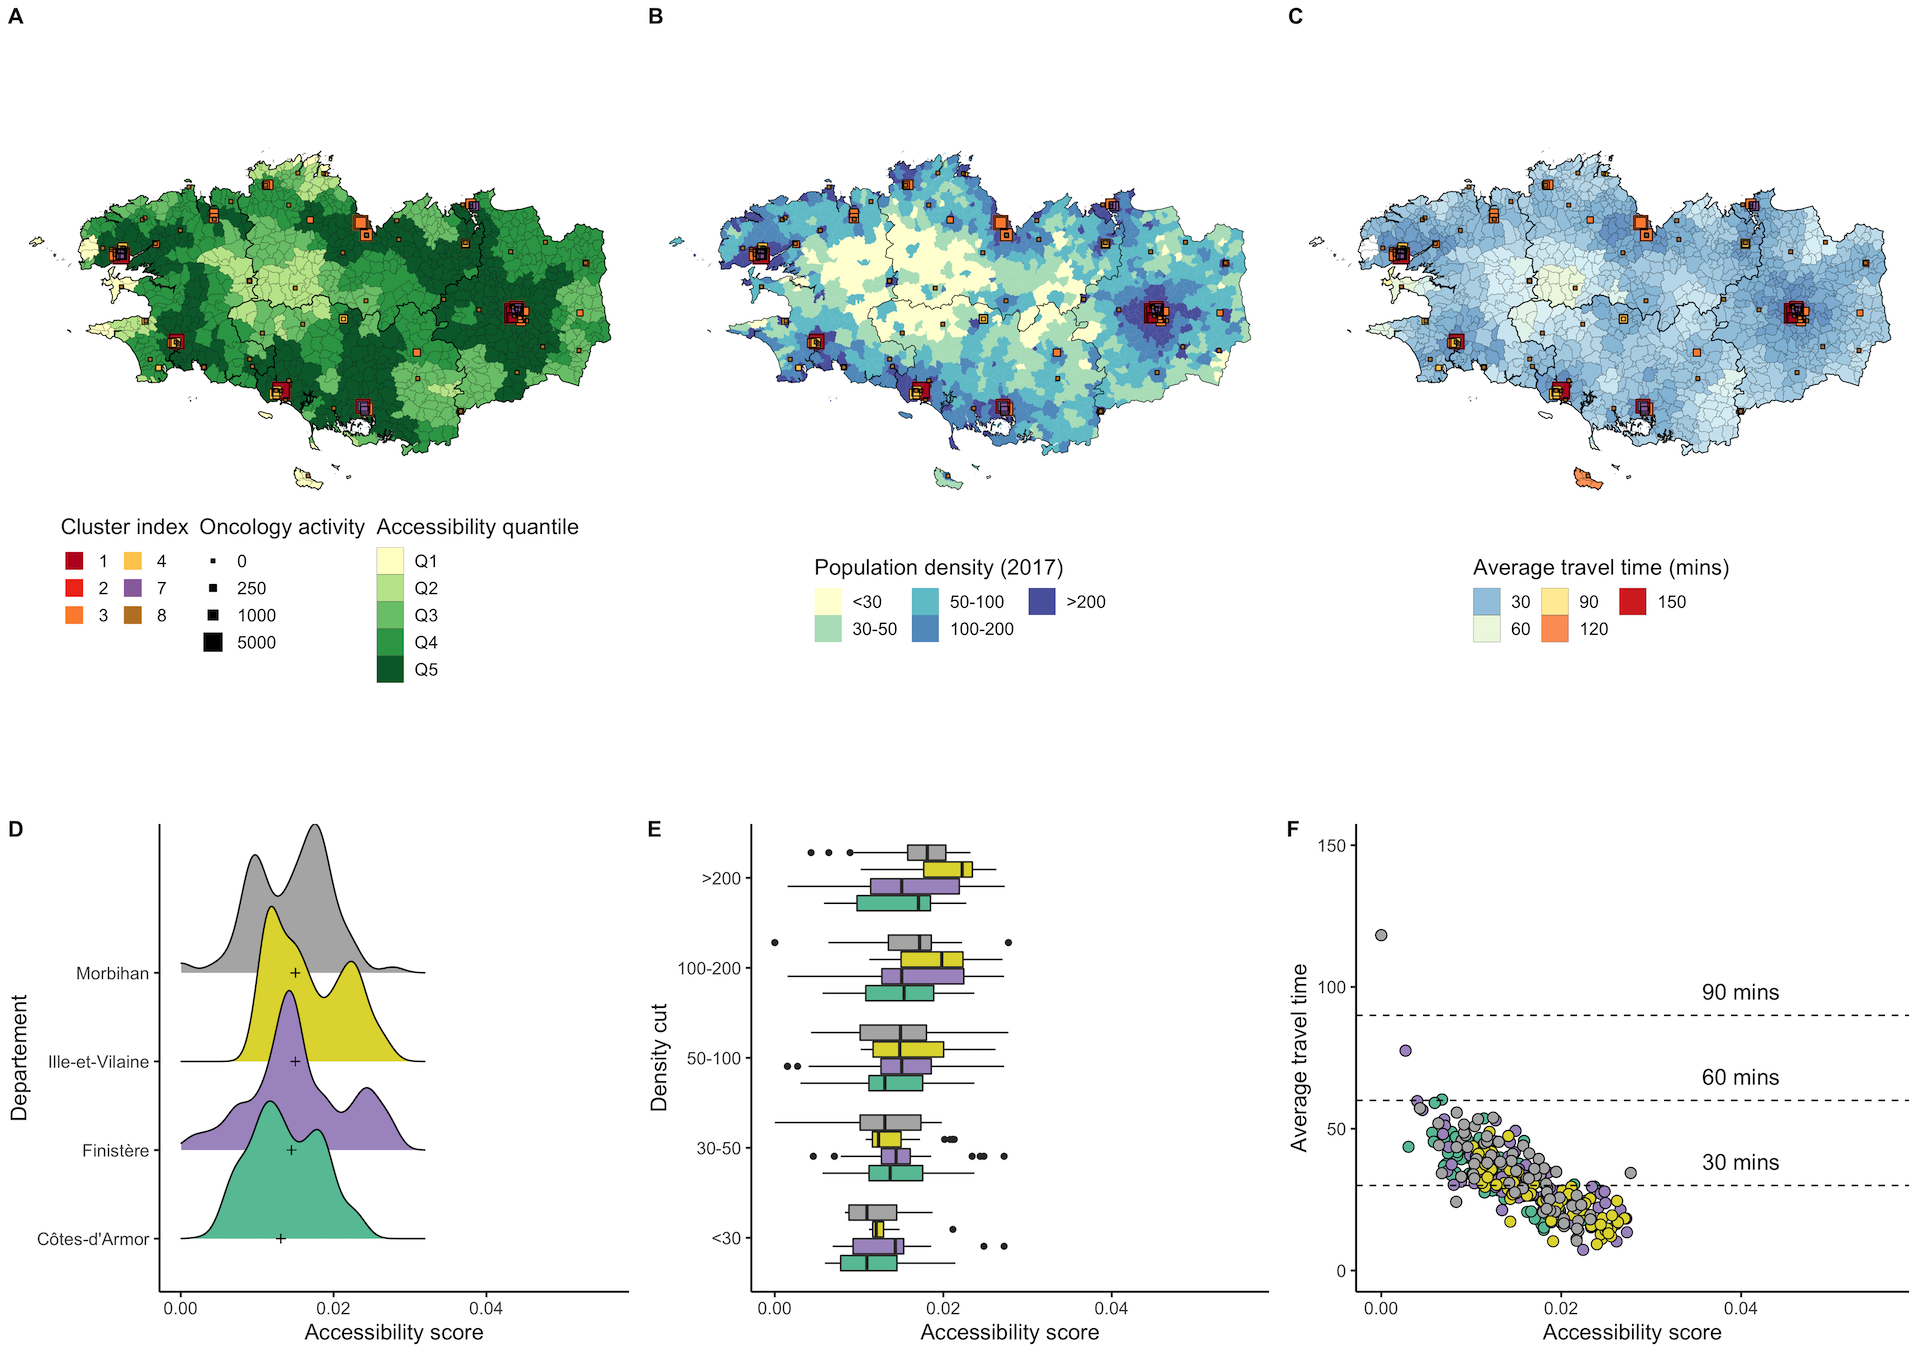
\includegraphics[width=\textwidth]{images/camion/region_accessibility/accessibility_Bretagne.png}
    \centering
    \caption{
        \textbf{Accessibility distribution in Bretagne.}
    }
\end{figure}

\subsection*{Bourgogne-Franche-Comté}

\begin{figure}[H]
    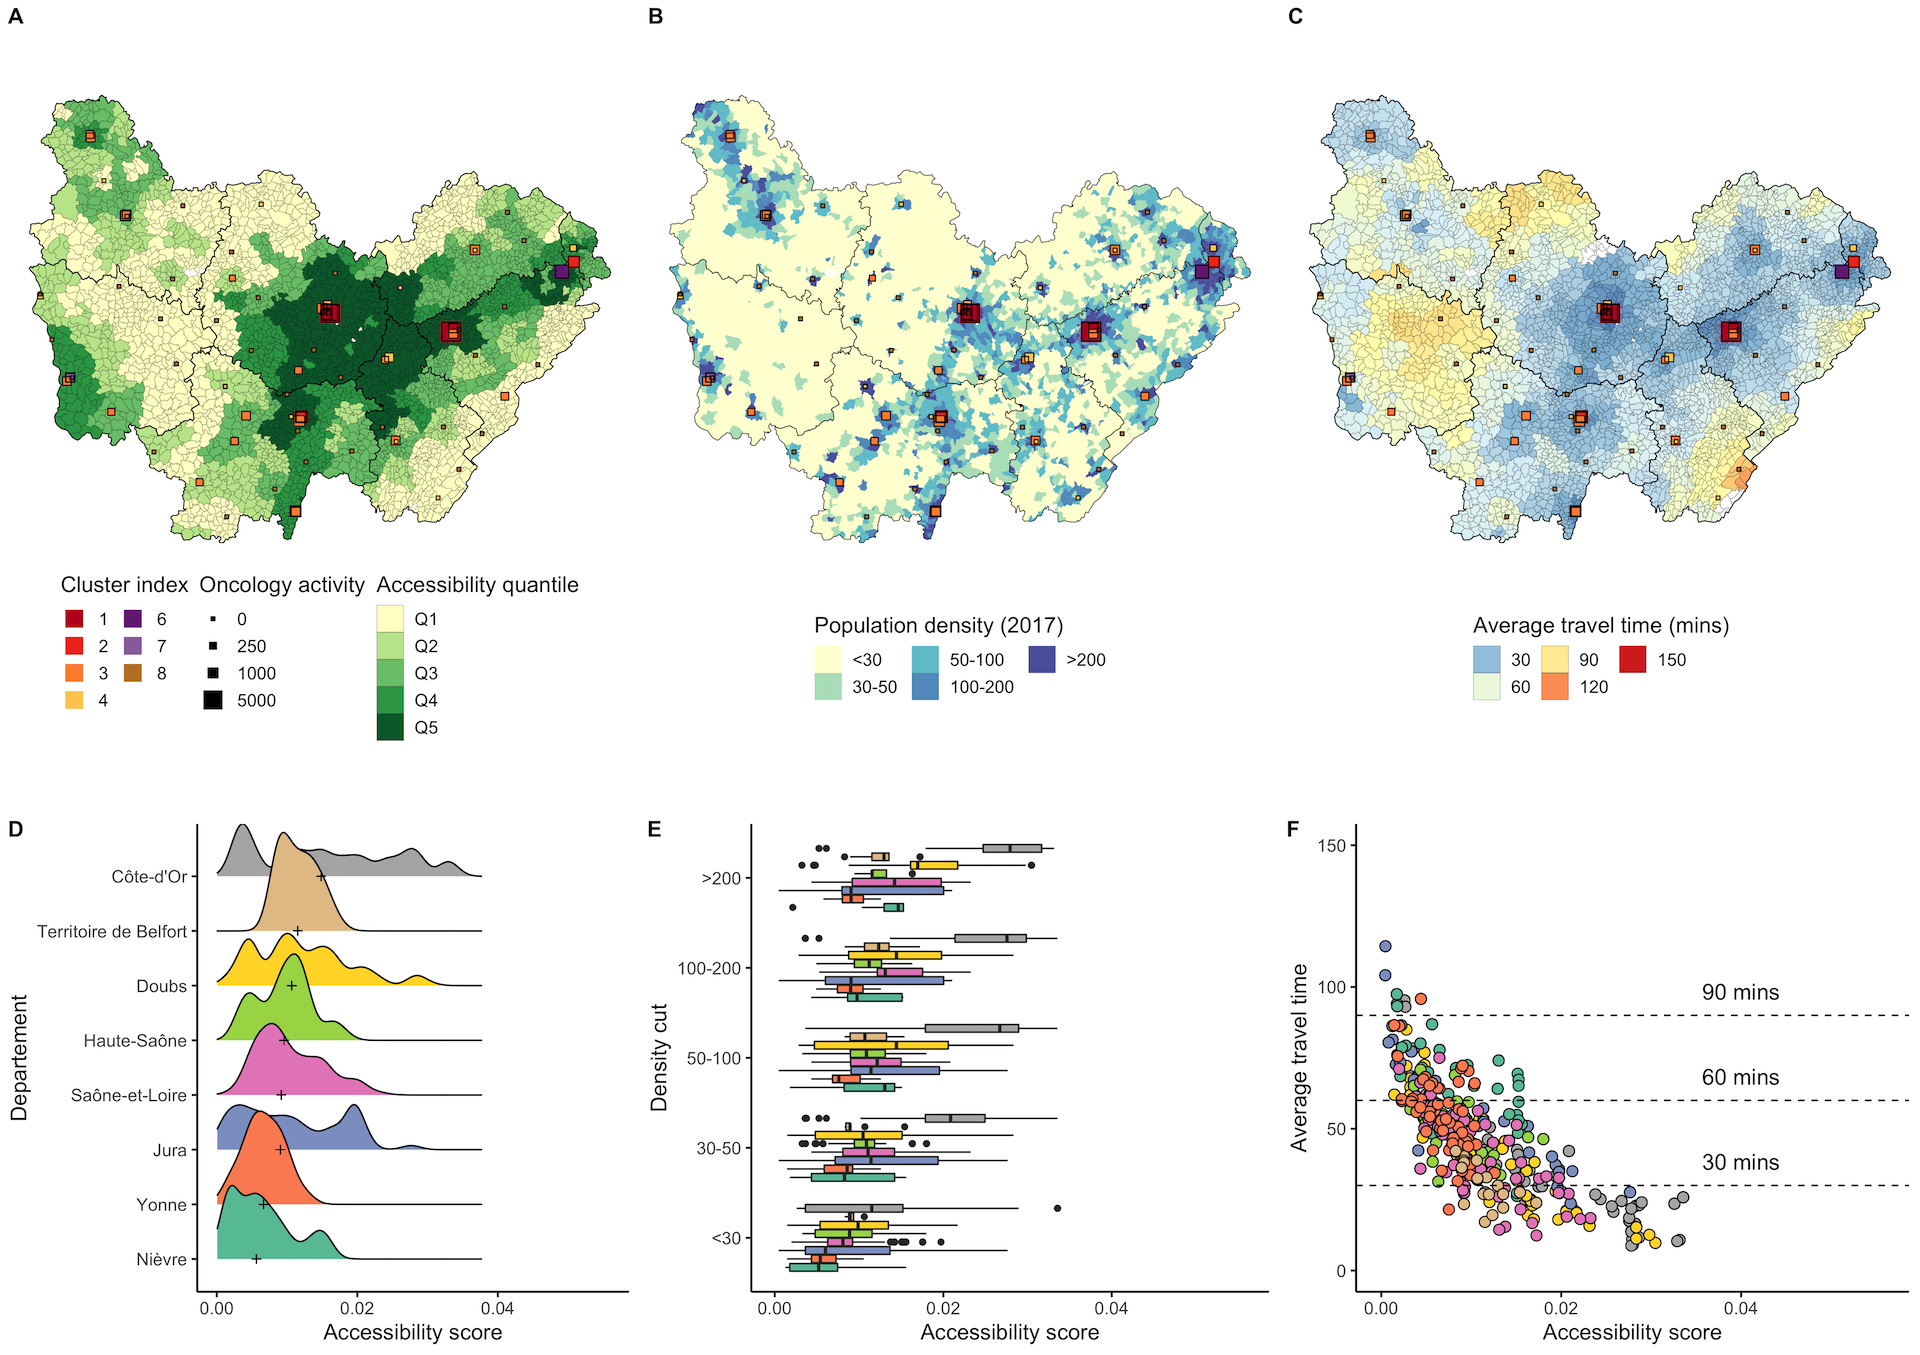
\includegraphics[width=\textwidth]{images/camion/region_accessibility/accessibility_Bourgogne-Franche-Comte.png}
    \centering
    \caption{
        \textbf{Accessibility distribution in Bourgogne-Franche-Comté.}
    }
\end{figure}

\subsection*{Auvergne-Rhône-Alpes}

\begin{figure}[H]
    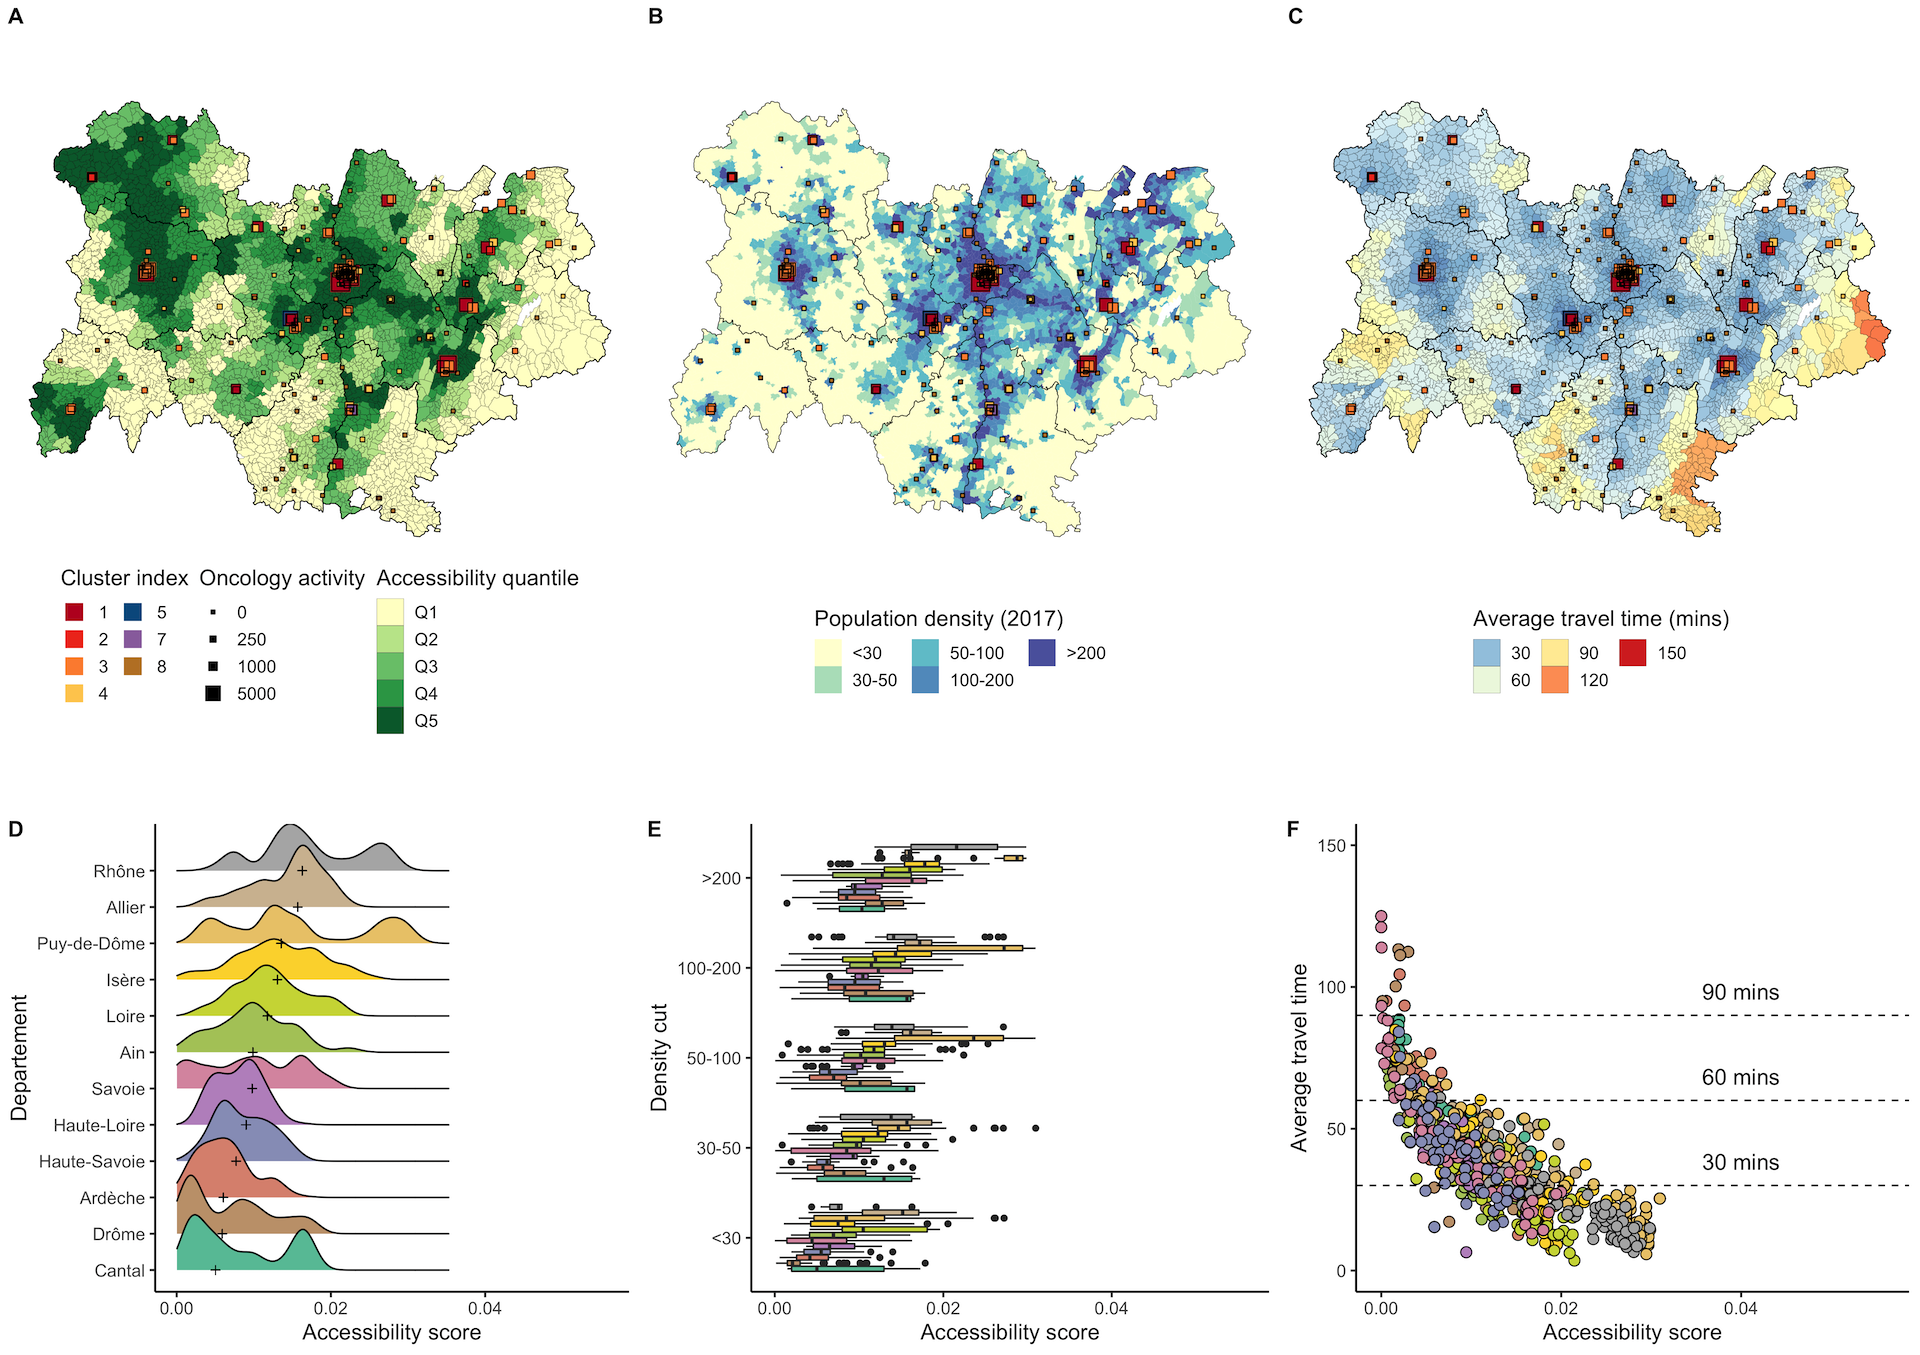
\includegraphics[width=\textwidth]{images/camion/region_accessibility/accessibility_Auvergne-Rhone-Alpes.png}
    \centering
    \caption{
        \textbf{Accessibility distribution in Auvergne-Rhone-Alpes.}
    }
\end{figure}

\section{Discussion}

Specific attention should be given to municipalities with very poor access to oncology care centers. While we saw that most of the population lives in high accessibility areas, around 6\% of the population lives in the bottom 20\% accessibility quantile. Among these municipalities, some are very rural and mountainous like those in the Alpes-de-Haute-Provence in Provence-Alpes-Cote-d'Azur region. Such areas cannot be expected to have a very good healthcare coverage. By contrast, the case of suburban areas with relatively dense population and poor accessibility should be addressed more easily. Our optimization algorithm can help driving public health policies, as it effectively identifies areas where accessibility could grow, by allocating additional oncology activity to a restricted number of care centers. The proposed growth factors are indicative and do not have to be effective within a year, as it represents a considerable effort for care centers to increase their activity.
Our oncology accessibility score is deliberately non-specific to cancer type. This score is meant to outline how easy it would be for a population location to reach a first entry point for oncology care. Here, we are only focusing on surgery, chemotherapy, and radiotherapy treatments. The same technique could be used on a specific cancer type, the method will remain the same, only the supply variable used in the accessibility score will change. We should mention that spatial accessibility is better suited for pathologies that are relatively well handled across the whole country. Accessibility for rare diseases like pediatric cancer or complex cancers that re-quire a specific expertise is less informative because only a handful of care centers are indicated.
Similarly, we could compute an accessibility score that is focused on specific kinds of stays: our web application lets the user pick between surgery, chemotherapy, or radiotherapy as supply variable.
